% Alex Pacini
% email: alexpacini90@gmail.com
% skype: alex_pacini
% blog: http://pacinispace.blogspot.com
%%
%%
\documentclass[a4paper]{report}
\usepackage[italian,english]{babel}
\usepackage[pdftex]{graphicx}
\usepackage[utf8x]{inputenc}
\usepackage[T1]{fontenc}
\usepackage{lmodern}
\usepackage{amssymb, amsmath, mathtools, cancel, mathrsfs}
\usepackage{float}
\usepackage{microtype, url}
\usepackage[bookmarks=true, hidelinks, pdftitle={EQUAZIONI DIFFERENZIALI LM},
pdfauthor={Alex Pacini}, pdfsubject={Appunti di Equazioni Differenziali LM,
Prof. Massimo Cicognani}, pdfkeywords={EQUAZIONI DIFFERENZIALI LM, Massimo
Cicognani, Ingegneria Elettronica e Telecomunicazioni per lo Sviluppo
Sostenibile}]{hyperref}
% If the package has not been installed into the LaTeX system files,
% manually specify the path to it like:
% \usepackage{./xx/xx/package}
%
\pagestyle{headings}
\graphicspath{{images/}}

%%%%%%%%%%%%%%%%% New Commands%%%%%%%%%%%%%%
%Integral from -\infty to +\infty
\newcommand{\intR}{\ensuremath{\int_{- \infty}^{+ \infty}}}
% Right arrow with spaces for follows statement
\newcommand{\follows}{\ensuremath{\;\;\; \Rightarrow \;\;\;}}
%Unit vectors
\newcommand{\uv}[1]{\ensuremath{\boldsymbol{\hat{#1}}}}
%i
\newcommand{\uvi}{\ensuremath{\uv{\imath}}}
%j
\newcommand{\uvj}{\ensuremath{\uv{\jmath}}}
%k
\newcommand{\uvk}{\ensuremath{\uv{k}}}
%Integral with the limit below(mathrlap)
\newcommand{\intlimr}[1]{\ensuremath{\int \limits_{\mathrlap{#1}}}}
%
\renewcommand{\phi}{\varphi}
%
%
%
%%%%%%%%%%%%%%%% End New Command %%%%%%%%%%%%
\begin{document}
\selectlanguage{italian}
%
\begin{titlepage}
\begin{center}
\vfill
%
{\LARGE{\sc Appunti di}}\\
\vspace{10mm} 
{\Huge {EQUAZIONI DIFFERENZIALI LM}} \\
\end{center}
%
\vspace{45mm}
\LARGE {E Dio disse...}
%
\begin{align*}
& \boldsymbol{\nabla} \cdot \boldsymbol{E} = \frac{\rho}{\varepsilon_0} \\
& \boldsymbol{\nabla} \cdot \boldsymbol{B} = 0 \\
& \boldsymbol{\nabla} \times \boldsymbol{E} = - \frac{\partial \boldsymbol{B}}{\partial t} \\
& \boldsymbol{\nabla} \times \boldsymbol{B} = \mu_0 \boldsymbol{J} + \varepsilon_0 \mu_0 \frac{\partial \boldsymbol{E}}{\partial t}
\end{align*}
%
\LARGE e la luce fu.
%
\vfill
\begin{center}
{\Large {Alex Pacini}}\\
\vspace{5mm}
{\large Cesena, \today}
\end{center}


\end{titlepage}

%
\null
\vfill
%
\selectlanguage{english}
	This work is licensed under the Creative Commons 
	Attribution-NonCommercial 3.0 Unported License.\\
	To view a copy of this license, visit 
	\url{http://creativecommons.org/licenses/by-nc/3.0/} or send a letter 
	to Creative Commons, 444 Castro Street, Suite 900, Mountain 
	View, California, 94041, USA.\\
	
	Alex Pacini
%
\selectlanguage{italian}
\newpage
\tableofcontents
\newpage
%
\chapter{Introduzione}	\label{chap:intro}
Partendo dalle leggi generali (conservazione, bilancio di massa, energia, ecc) e dalle leggi costitutive si andranno a definire
i vari modelli matematici composti dall'equazione (o sistema di equazioni) alle derivate parziali che governano i vari fenomeni fisici associati.
Attraverso l'imposizione di condizioni iniziali e/o condizioni al contorno si dimostra l'esistenza, l'unicit\`a della soluzione e la dipendenza continua
dai dati iniziali.
%%%%%%%%%%%%%%%%%%%%%%%%%%%%%%%%%%%%%%%%%%%%%%%%%%%%%%%%%%%%%%%%%%%
\section{\texorpdfstring
{Classificazione delle Equazioni di II ordine in due variabili ($t,x$)}
{Classificazione delle Equazioni di II ordine in due variabili (t,x)}}
La forma completa di un' equazioni di II ordine in due variabili pu\`o essere espressa come segue
\[
	\underbrace{au_{tt}+2bu_{xt}+cu_{xx}}_\text{parte principale} + 
	du_t + eu_x + hu = f
\]
con $a>0$.
Considerando quindi la parte principale e sostituendo la derivata rispetto a $t$ con la variabile simbolica $p$ mentre la derivata 
rispetto a $x$ con $q$, si pu\`o scrivere
\[
	ap^2 + 2bpq + cq^2 = tr(AH)
\]
dove $A$ \`e la matrice associata all'equazione differenziale e $H$ \`e la matrice Hessiana di $u$.
\[
A=
 \begin{pmatrix}
  a & b \\
  b & c
 \end{pmatrix}
\;\;\;
%%%%%%%%%%%%%%%%%%%%%%%%%%%%%%%%%%%%%%%%%%%%%%%%%%%%%%%%%%%%%%%%%%%
H=
 \begin{pmatrix}
  \partial_{tt} & \partial_{tx} \\
  \partial_{xt} & \partial_{xx}
 \end{pmatrix}
\]
\`E ora possibile classificare le equazioni differenziali in base alla matrice $A$.
%
\begin{align*}
& A \mbox{ indefinita }  \Rightarrow  \mbox{ iperbolica}\\
& A \mbox{ semidefinita positiva }  \Rightarrow  \mbox{ parabolica}\\
& A \mbox{ definita positiva }  \Rightarrow  \mbox{ ellittica}
\end{align*}
%
Infatti, definito $\Delta=b^2-4ac$, se
%
\begin{align*}
& \Delta>0 \Rightarrow tr(AH)=1 \mbox{ indica un iperbole }\\
& \Delta=0 \Rightarrow tr(AH)=1 \mbox{ indica una parabola }\\
& \Delta<0 \Rightarrow tr(AH)=1 \mbox{ indica un'ellisse }
\end{align*}
%
La classificazione si estende in maniera naturale ad equazioni in $n>2$ variabili.

{\bf Esempi noti}
\[
\begin{array}{ll}
	u_t - Du_{xx}=f &\mbox{ eq. della diffusione: parabolica }\\
	u_{tt} + u_{xx}=f &\mbox{ eq. di Laplace: ellittica }\\
	u_{tt} - c^2 u_{xx}=f &\mbox{ eq. delle onde: iperbolica }
\end{array}
\]
Un'equazione pu\`o anche essere di tutti e tre i tipi, ne \`e un esempio l'equazione di Eulero-Tricomi ($u_{tt}-tu_{xx}=f$), che per $t>0$ \`e iperbolica,
per $t=0$ parabolica e per $t<0$ ellittica. 
%
\chapter{Equazione della Diffusione (Paraboliche)}	\label{chap:diffusion}
\section{Derivazione dell'equazione del calore}
Definiamo innanzitutto le variabili in gioco:\\
$t=$ tempo, $x=$ posizione, $u(t,x)=$ temperatura nella posizione $x$ e al tempo $t$.\\
Nel definire il modello si far\`a uso di:
%
\begin{align*}
& r= \mbox{ tasso di calore per unit\`a di massa dall'esterno } \; [r]=\frac{[cal]}{[tempo][massa]}\\
& \rho= \mbox{ densit\`a (lineare) di massa della barra } \; [\rho]=\frac{[massa]}{[lunghezza]}\\
& q= \mbox{ flusso di calore } \; [q]=\frac{[cal]}{[tempo]}\\
& e= \mbox{ energia interna per unit\`a di massa } \; [r]=\frac{[cal]}{[massa]}\\
\end{align*}

Il primo passo nella derivazione dell'equazione del calore consiste nell'applicare la \textit{Legge di Bilancio}:\\
isolata una porzione $[x_0, x_0+h]$ della barra, il tasso di variazione dell'energia interna eguaglia il flusso agli estremi;
nel caso di sorgente, il tasso di variazione del calore erogato sar\`a sommato al flusso agli estremi.
\[
	\underbrace{\frac{d}{dt}\int_{x_0}^{x_0+h} e(t,x)\rho dx}_\text{Variazione dell'energia rispetto al tempo}
	= \overbrace{q(t,x_0)-q(t,x_0 +h)}^\text{Flusso entrante}
	+\underbrace{\int_{x_0}^{x_0+h} r(t,x) \rho dx}_\text{Flusso della sorgente}
\]
Per il Teorema Fondamentale del Calcolo Integrale
\[
	q(t,x_0)-q(t,x_0 +h) = -\int_{x_0}^{x_0+h} q_x(t,x)dx
\]
dove $q_x$ indica $\frac{dq}{dx}$.

Considerando che l'espressione 
\[
	\frac{d}{dt}\int_{x_0}^{x_0+h} e(t,x)\rho dx
	= -\int_{x_0}^{x_0+h} q_x(t,x)dx
	+\int_{x_0}^{x_0+h} r(t,x) \rho dx
\]
deve essere valida per $x_0$ e $x_0+h$ e che, data la continuit\`a dell'energia \`e possibile portare 
la derivata all'interno del segno di integrale, si ottiene la Legge di Bilancio in forma locale
\[
	\frac{\partial}{\partial t} e(t,x)\rho= -\frac{\partial}{\partial x}q(t,x)+\rho r(t,x)
\]

\`E ora necessario applicare le leggi costitutive, che risultano essere delle leggi sperimentali.\\
La prima, che prende il nome di \textit{Legge di Fourier}, indica che il flusso di calore ($q$) \`e direttamente proporzionale
alla derivata spaziale della temperatura secondo la legge
\[
	q= -ku_x
\]
con $u=u(t,x)$ e $k>0$. Il segno negativo indica che si ha il flusso positivo passando dalla zona pi\`u calda a quella pi\`u fredda.
\[
	[k]= \frac{[cal]}{[tempo]}\frac{[lunghezza]}{[grado]}
\]
La seconda lega invece l'energia alla temperatura
\[
	e= c_lu
\]
dove $c_l$ indica il calore specifico ed \`e $>0$
\[
	[c_l]=\frac{[cal]}{[massa][grado]}
\]
Operando la sostituzione si ottiene
\[
	\rho c_l \frac{\partial}{\partial t} u= k \frac{\partial^2}{\partial x^2}u + \rho r
\]
che riordinata
\[
	u_t= \underbracket{D}_{\mathclap{\text{Risposta termica}}} u_{xx}+f
\]
dove $D=k/c_l\rho$ e $f=r/c_l$.
\[
	[D]=\frac{\cancel{[cal]}[lunghezza]}{[tempo]\cancel{[grado]}}\frac{\cancel{[massa]}\cancel{[grado]}}{\cancel{[cal]}}
	\frac{[lunghezza]}{\cancel{[massa]}}=\frac{[lunghezza]^2}{[tempo]}
\]

L'equazione caratteristica risulta quindi essere, considerata l'equazione differenziale omogenea e sostituendo due variabili algebriche alle due variabili derivate
\[
	u_t= Du_{xx} \;\;\; \Rightarrow \;\;\; T=DX^2
\]
Si noti che \`e l'equazione di una parabola.
%%%%%%%%%%%%%%%%%%%%%%%%%%%%%%%%%%%%%%%%%%%%%%%%%%%%%%%%%%%%%%%%%%%%%%%%%%%%%%%%%%%%%%%%%%%%%%%%%%%%%%%%%%%
\section{Problemi ``Ben Posti''}
%
\chapter{Equazione di Laplace (Ellittiche)}		\label{chap:laplacian}
\section{Introduzione}
L'equazione di diffusione in un corpo bidimensionale \`e
\[
	u_t= D(u_{xx}+ u_{yy} +f)
\]
mentre in un corpo a tre dimensioni (solido) \`e
\[
	u_t=D\left( u_{xx}+u_{yy} +u_{zz} \right) +f
\]
L'operatore 
\[
	\Delta= \partial_{x_1x_1}+ \ldots + \partial_{x_n x_n}
\]
in ogni dimensione $n$ \`e detto \textit{Laplaciano}. Con questa notazione
l'equazione di diffusione si scrive 
\[
	u_t= D\Delta u +f
\]
Nel caso di sorgenti $f$ non dipendenti dal tempo, \`e ragionevole cercare 
soluzioni stazionarie, cio\`e anch'esse indipendenti da $t$.
Si giunge cos\`i all'\textit{equazione di Poisson}
\[
	\Delta u= -f/D
\]
Nel caso omogeneo $f=0$, l'equazione
\[
	\Delta u=0
\]
si dice \textit{equazione di Laplace} e le soluzioni si dicono 
\textit{funzioni armoniche}.\\
Anche le soluzioni stazionarie dell'equazione
\[
	u_{tt}c^2 \Delta u
\]
sono funzioni armoniche. In dimensione di spazio $n=2$, questa equazione
descrive lo spostamento di una membrana elastica dalla posizione di riposo.
Una posizione stazionaria (equilibrio) \`e quindi descritta da una funzione
armonica.
Se $F=(f_1,f_2, f_3)=f_1= f_1 \uvi + f_2 \uvj + f_3 \uvk$ \`e un campo
vettoriale nello spazio, la divergenza di $F$ \`e lo scalare
\[
	div F= \partial_x f_1 + \partial_y f_2 + \partial_z f_3
\]
Se esiste una funzione scalare $u$ tale che
\[
	\nabla u= F
\]
(potenziale), allora
\[
	div F= div \nabla u = div \left( u_x \uvi +u_y \uvj + u_x \uvk \right)
	=\Delta u
\]
L'equazione di Laplace/Poisson \`e quindi fondamentale nello studio dei campi conservativi. Se $E$ \`e un campo elettrostatico in una regione $\Omega$
di spazio, allora si ha
\[
	div E= \frac{4 \pi \rho}{\varepsilon}
\]
con $\rho$ densit\`a di carica ed $\varepsilon$ costante dielettrica. Se
\[
	\Delta u= -E
\]
il potenziale soddisfa l'equazione di Poisson
\[
	\Delta u= - \frac{4 \pi \rho}{\varepsilon}
\]
Nel caso $\rho=0$, cariche fuori di $\Omega$, la funzione $u$ \`e armonica.
In dimensione $n=2$, le funzioni armoniche intervengono anche nello studio
di funzioni di variabile complessa.
Se $f= u+iv$ \`e derivabile in senso complesso, vale l'equazione di 
Cauchy- Riemann
\[
	\frac{\partial f}{\partial x}= \frac{1}{i} \frac{\partial f}
	{\partial y}
\]
che si scrive anche 
\[
	\left\{ 
	\begin{array}{l}
		u_x=v_y \\
		v_x=- u_y
	\end{array}
	\right.
\]
Dunque
\[
	\Delta u= u_{xx}+ u_{yy}= v_{yx}-v_{xy}=0
\]
\[
	\Delta v= v_{xx}+ v_{yy}= -u_{yx} +u_{xy}=0
\]
La parte reale $u$ e l parte immaginaria $v$ di $f$ sono funzioni
armoniche.
Viceversa, se $u$ \`e una funzione armonica, \`e possibile risolvere le
equazioni di Cauchy-Riemann rispetto a $v$ in ogni parte semplicemente connessa
del dominio in modo che 
\[
	f= u+ iv
\]
sia una funzione derivabile in senso complesso.
Tale funzione \`e in realt\`a derivabile infinite volte perch\'e si pu\`o
espandere localmente in serie di potenze. Ne segue che $u$ (e $v$) \`e
derivabile infinite volte in $dx$, $dy$.
Abbiamo cos\`i che una funzione armonica nel piano \`e derivabile infinite
cio\`e di classe $C^{\infty}$.
\section{Formule di Gauss-Green ed applicazioni al Laplaciano}
Se $\gamma$ \`e una curva chiusa nel piano, orientata in senso antiorario,
regolare (a tratti) con parametrizzazione
\[
	x= x(t), \;\;\; y=y(t), \;\;\; a\leq t \leq b
\]
Il versore tangente a $\gamma$
\[
	{\bf T}= \frac{1}{\sqrt{(x')^2+ (y')^2}}(x', y')
	=\frac{x'}{\sqrt{(x')^2+ (y')^2}}\uvi
	+\frac{y'}{\sqrt{(x')^2+ (y')^2}}\uvj
\]
Ora, per ottenere il versore normale ${\bf N}$, bisogna calcolare il versore
ortogonale a ${\bf T}$; ci\`o \`e ottenuto con
\[
	{\bf N}= \frac{1}{\sqrt{(x')^2+ (y')^2}}(y', -x')
	=\frac{y'}{\sqrt{(x')^2+ (y')^2}}\uvi
	-\frac{x'}{\sqrt{(x')^2+ (y')^2}}\uvj
\]
che rappresenta la normale esterna a $\gamma$; la normale interna \`e invece
\[
	{\bf N}= \frac{1}{\sqrt{(x')^2+ (y')^2}}(-y', x')
	=-\frac{y'}{\sqrt{(x')^2+ (y')^2}}\uvi
	+\frac{x'}{\sqrt{(x')^2+ (y')^2}}\uvj
\]
Dato un campo vettoriale $F= f_1 \uvi + f_2 \uvj$, gli integrali curvilinei
\[
	\int_ {\gamma} F \cdot {\bf T} ds= 
	\int_a^b \left[ f_1 (x(t), y(t))x'(t)+
	f_2 (x(t), y(t))y'(t)
	\right] dt
\]
\[
	\int_ {\gamma} F \cdot {\bf N} ds= 
	\int_a^b \left[ f_1 (x(t), y(t))y'(t)
	- f_2 (x(t), y(t))x'(t)
	\right] dt
\]
rappresentano, rispettivamente, il lavoro di $F$ su $\gamma$ ed il flusso
uscente di $F$ da $\Omega$. Si \`e fatto uso dello spostamento infinitesimo
\[
	ds= \sqrt{(x')^2+(y')^2}
\]

Le formule di Gauss-Green collegano gli integrali curvilinei su $\gamma$
ad integrali in $dx dy$ su $\Omega$:
\[
	\int_{\Omega}\partial_x f(x,y)dx dy= \int_{\gamma} f \uvj \cdot {\bf T} ds
\]
\[
	\int_{\Omega}\partial_y f(x,y)dx dy= - \int_{\gamma} f \uvi \cdot {\bf T} ds
\]
Tali formule sono di facile dimostrazione su domini normali. Ad esempio
preso $\Omega$ come in fig. \ref{nor_dom}
\begin{figure}[H]
	\centering
	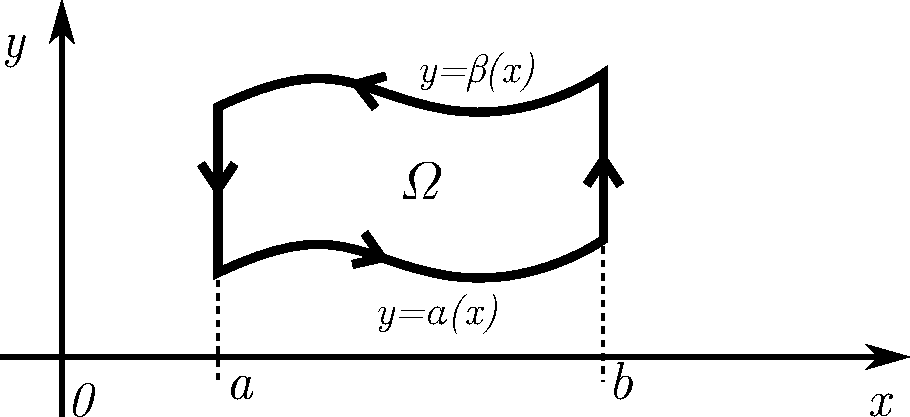
\includegraphics[width=0.8\textwidth]{nor_dom.pdf}
	\caption{Dominio normale per la dimostrazione delle formule di Green}
	\label{nor_dom}
\end{figure}
\noindent
si ha
\[
	\int_{\Omega} \partial_y f (x,y) dx dy=
	\int_a^b \int_{\alpha(x)}^{\beta(x)}
	\partial_y f (x,y) dx dy=
	\int_a^b \left[
		f(x,y)
	\right]_{y=\alpha(x)}^{y=\beta(x)}dx
\]
\[
	= \int_a^b \left[
	f(x,\beta (x)) - f(x, \alpha(x))
	\right] dx
\]
Per il tratto di frontiera
\[
	\left\{ 
	\begin{array}{ll}
		x=x & x \in [a,b] \\
		y= \alpha(x)
	\end{array}
	\right.
\]
si ha
\[
	{\bf T}= \frac{1}{\sqrt{1+ (\alpha ' )^2}}(1,\alpha ')
\]
\[
	ds= \sqrt{1+ (\alpha ' )^2} dx
\]
\[
	{\bf T} \cdot \uvi ds= dx
\]
perci\`o
\[
	\int \limits_{\gamma_{[a,b]}} f(x,y)\uvi \cdot {\bf T} ds
	= \int_a^b f(x, \alpha(x)) dx
\]
Per il tratto orientato in senso contrario
\[
	\left\{ 
	\begin{array}{ll}
		x=x & x \in [b,a] \\
		y= \beta(x)
	\end{array}
	\right.
\]
si ha
\[
	{\bf T}= - \frac{1}{\sqrt{1+ (\beta ' )^2}}(1,\beta ')
\]
\[
	ds= \sqrt{1+ (\beta ' )^2} dx
\]
\[
	{\bf T} \cdot \uvi ds= -dx
\]
perci\`o
\[
	\int \limits_{\gamma_{[b,a]}} f(x,y)\uvi \cdot {\bf T} ds
	= \int_b^a f(x, \beta(x)) dx
	= -\int_a^b f(x, \beta(x)) dx
\]
Nei due tratti verticali si ha ${\bf T} = \pm \uvj$, 
quindi ${\bf T} \cdot \uvi = 0$.\\
Per concludere
\[
	\int_{\gamma} f(x,y)\uvi \cdot {\bf T} ds = 
	\int_a^b f(x, \alpha(x)) dx
	- \int_a^b f(x, \beta(x)) dx=
\]
\[
	- \int_a^b \left[ f(x, \beta(x)) -f(x, \alpha(x)) \right] dx
\]
e quindi
\[
	\int_{\gamma} f(x,y)\uvi \cdot {\bf T} ds =
	- \int_{\Omega} \partial_y f (x,y) dx dy=
\]
Il teorema diventa estendibile anche a domini non normali, data la possibilit\`a di scomporre un dominio qualsiasi in domini normali.

Analoga dimostrazione pu\`o essere fatta per la formula restante, in questo 
caso utilizzando un dominio perpendicolare all'asse y.

Per un campo $F= f_1 \uvi + f_2 \uvj$ si ottiene
\[
	\int_{\gamma} F \cdot {\bf T} ds
	= \int_{\gamma} f_1 \uvi \cdot {\bf T} ds
	+ \int_{\gamma} f_2 \uvj \cdot {\bf T} ds
	= \int_{\Omega} (\partial_x f_2 - \partial_y f_1)dxdy
\]
cio\`e la formula di Stokes
\[
	\int_{\gamma} F \cdot {\bf T} ds
	= \int_{\Omega} (\partial_x f_2 - \partial_y f_1)dxdy
\]
nel piano. L'integrale doppio pu\`o essere visto come il flusso attraverso la
superficie piana $\Omega$ di $rot F$ pensando ad $F= f_1 \uvi + f_2 \uvj +0\uvk$ nello spazio.\\
Inoltre, ricordando che
\[
	{\bf N} \cdot \uvi= {\bf T} \cdot \uvj, \;\;\;
	{\bf N} \cdot \uvj= -{\bf T} \cdot \uvi
\]
si ha
\[
	\int_{\gamma} F \cdot {\bf N} ds=
	\int_{\gamma} f_1 \uvi \cdot {\bf N} ds +
	\int_{\gamma} f_2 \uvj \cdot {\bf N} ds =
	\int_{\gamma} f_1 \uvj \cdot {\bf T} ds -
	\int_{\gamma} f_2 \uvi \cdot {\bf T} ds =
\]
\[
	\int_{\Omega} \left( \partial_x f_1 + \partial_y f_2 \right)dxdy
\]
che \`e il teorema della divergenza nel piano
\[
	\int_{\gamma} F \cdot {\bf N} ds=
	\int_{\Omega} div F \; dxdy
\]
Le formule di Gauss-Green e le loro conseguenze forniscono importati applicazioni
al Laplaciano.

Per $F= \nabla u$, il teorema della divergenza diventa
\[
	\int_{\Omega} \Delta u \; dxdy=
	\int_{\gamma} \nabla u \cdot {\bf N} ds =
	\int_{\gamma} \partial_{\bf N} u \; ds
\]
in quanto $\nabla u \cdot {\bf N}$ coincide con la derivata
$ \partial_{\bf N} u$ lungo la normale esterna.\\
Applicando poi il teorema della divergenza al campo
\[
	vF= vf_1 \uvi + vf_2 \uvj
\]
si ha
\[
	div(vF)= v_x f_1 + v_y f_2 + 
	v \left( \frac{\partial}{\partial_x} f_1 
	+ \frac{\partial}{\partial_y} f_2 \right)
\]
\[
	= \nabla v \cdot F + v\, divF
\]
perci\`o
\[
	\int_{\gamma} vF \cdot {\bf N} ds =
	\int_{\Omega} div(vF) \; dxdy=
	\int_{\Omega} \nabla v \cdot F \; dxdy +
	\int_{\Omega} v\, divF \; dxdy
\]
Questa, con $F= \nabla u$, si riduce a
\[
	\int_{\gamma} v \, \partial_{\bf N} u \; ds =
	\int_{\Omega} \nabla v \cdot \nabla u \; dxdy +
	\int_{\Omega} v\, \Delta u \; dxdy
\]
che conviene mettere nella forma di integrale per parti per il Laplaciano
\[
	\int_{\Omega} v\, \Delta u \; dxdy =
	\int_{\gamma} v \, \partial_{\bf N} u \; ds -
	\int_{\Omega} \nabla v \cdot \nabla u \; dxdy
\]
\section{Problemi ben posti}
Sia $\Omega$ un dominio limitato di $\mathbb{R}^2$ con frontiera $\gamma$
curva chiusa regolare a tratti orientata in senso positivo.
I problemi ben posti per l'equazione $\Delta u= f$ in $Omega$ sono quelli
visti per la diffusione, senza dato iniziale mancando la variabile tempo.\\
Per il problema di Dirichlet:
\[
	\left\{
	\begin{array}{ll}
		\Delta u= f & \text{in} \;\;\; \Omega \\
		u= g & \text{in} \;\;\; \gamma
	\end{array}
	\right.
\]
Per il problema di Neumann:
\[
	\left\{
	\begin{array}{ll}
		\Delta u= f & \text{in} \;\;\; \Omega \\
		\partial_{\bf N}u= h & \text{in} \;\;\; \gamma
	\end{array}
	\right.
\]
La formula
\[
	\int_{\Omega} \Delta u \; dxdy=
	\int_{\gamma} \partial_{\bf N} u \; ds
\]
fornisce una condizione di compatibilit\`a tra la sorgente $f$ ed il flusso
uscente $h$ nel problema di Neumann. La condizione necessaria per l'esistenza
di soluzioni \`e
\[
	\int_{\Omega} f \; dxdy=
	\int_{\gamma} h \; ds
\]

\section{Unicit\`a}
Si mostra che i problemi con dati iniziali coincidenti hanno la stessa
soluzione.\\
Se $u_1$ $u_2$ sono due soluzioni allora
\[
	w=u_1- u_2
\]
risolve 
\[
	\Delta w = 0 \;\;\; \text{in} \;\;\; \Omega
\]
con condizioni al contorno
\[
	\begin{array}{lll}
		w=0 & \text{in } \gamma & \text{Dirichlet}\\
		\partial_{\bf N}w=0 & \text{in } \gamma & \text{Neumann}\\
	\end{array}
\]
Sostituendo $u=v=w$ nella formula dell'integrale per parti 
(equivalente ad usare il campo $div\, (ww)= div\, w^2$)
\[
	\int_{\Omega} w \Delta w \, dxdy= 
	- \int_{\Omega} \nabla w \cdot \nabla w \, dxdy
	+ \int_{\gamma} w \partial_{\bf N} w \, ds
\]
il termine
\[
	\int_{\gamma} w \partial_{\bf N} w \, ds
\]
\`e nullo sia con condizioni di Neumann nulle ($\partial_{\bf N} w =0 $) sia
con le condizioni di Dirichlet nulle ($w=0$).
Perci\`o, data la definizione $\Delta w= 0$,
\[
	0= - \int_{\Omega} \left|\left| \nabla w \right|\right|^2 \, dxdy +0
\]
\[
	\int_{\Omega} \left|\left| \nabla w \right|\right|^2 \, dxdy = 0
\]
L'unica soluzione, essendo somma di quadrati, \`e 
\[
	\nabla w=0
\]
in $\Omega$. Quindi
\[
	w=C \;\;\; \text{in} \;\;\; \Omega
\]
Questo pone l'unicit\`a a meno di costanti nel caso di Neumann.\\
Per Dirichlet deve essere $w=c=0$ in $\gamma$ (o almeno $\gamma_0$),
quindi $w=0$ ovunque nella chiusura $\bar{\Omega}= \Omega \cup \gamma$ di $\Omega$.
\section{Propriet\`a di media}
Sia $u(x,y)$ armonica in $\Omega \leq \mathbb{R}^2$
\[
	\Delta u= 0 \;\;\; \text{in} \;\;\; \Omega
\]
Denotiamo con $\Omega_R(x,y)$ un generico cerchio di centro $(x,y)$ e raggio
$R$ contenuto in $\Omega$ e con $\gamma_R(x,y)$ la circonferenza di frontiera
orientata positivamente.
\begin{figure}[H]
	\centering
	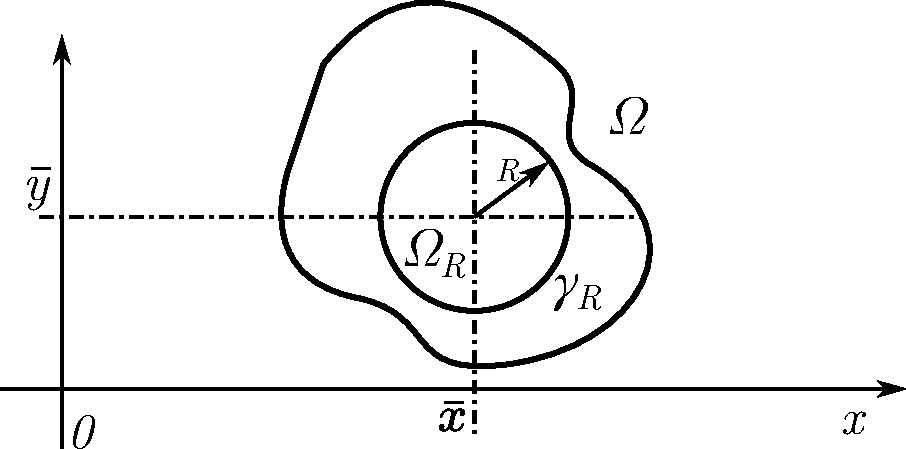
\includegraphics[width=0.8\textwidth]{mean_f.pdf}
	\caption{Circonferenza di frontiera $\gamma_R$}
	\label{mean_f}
\end{figure}
\noindent
\subsection{Formule di media}
In tale dominio circolare valgono le formule di media
\[
	u(\bar{x}, \bar{y})= \frac{1}{\pi R^2}
	\int \limits_{\Omega_R}
	u(x,y) \, dxdy
\]
\[
	u(\bar{x}, \bar{y})= \frac{1}{2 \pi R}
	\int \limits_{\gamma_R}
	u \, ds
\]
con $ds$ l'elemento di lunghezza sulla circonferenza.
\subsubsection{Dimostrazione}
Iniziamo dalla seconda. Per $0<\pi<R$ poniamo 
\[
	g(r)= \frac{1}{2\pi r}
	\int \limits_{\gamma_r}
	u \, ds=
	\frac{1}{2\pi r}
	\int_0^{2\pi}
	u(\bar{x}+rcos \theta, \bar{y} + rsin \theta) \, r d\theta
\]
\[
	= \frac{1}{2\pi}
	\int_0^{2\pi}
	u(\bar{x}+rcos \theta, \bar{y} + rsin \theta) \, d\theta
\]
dove si \`e usata la parametrizzazione di $\gamma_r(x,y)$
\[
	\left\{
		\begin{array}{l}
			x= \bar{x} + rcos\theta \\
			y= \bar{y} + rsin\theta
		\end{array}
	\right.
\]
con $0 \leq \theta \leq 2\pi$.\\
Dove $x'=-rsin \theta$, $y'= rcos \theta$, $ds= \sqrt{(x')^2+ (y')^2}= rd\theta$.\\
Derivando $g(r)$ abbiamo
\[
	g'(r)= \frac{1}{2\pi}
	\int_0^{2\pi} 
	\left(
		u_x cos\theta + u_y sin \theta
	\right)d\theta=
	\frac{1}{2\pi r}
	\int \limits_{\gamma_r} \nabla u \cdot {\bf N} ds
\]
dove si \`e usato
\[
	{\bf N} = cos\theta \uvi + sin \theta \uvj , \;\;\;
	d\theta= \frac{ds}{r}
\]
Per il teorema della divergenza
\[
	\frac{1}{2\pi r}
	\int \limits_{\gamma_r} \nabla u \cdot {\bf N} ds=
	\int \limits_{\Omega_r} div (\nabla u) dxdy=
	\int \limits_{\Omega_r} \Delta u \, dxdy= 0
\]
cio\`e $g(r)$ costante.\\
Poich\'e 
\[
	\lim_{r \to 0} g(r)=
	\lim_{r \to 0} \frac{1}{2 \pi}
	\int_0^{2\pi} 
	u(\bar{x}+rcos \theta, \bar{y} + rsin \theta) \, d\theta=
	\frac{1}{2 \pi} \int_0^{2\pi}
	u(\bar{x}, \bar{y}) d\theta
\]
\[
	= u(\bar{x}, \bar{y})
\]
abbiamo
\[
	g(r)= u(\bar{x}, \bar{y}) \;\;\; \text{per ogni} \;\;\; r \in (0,R]
\]
il ch\'e prova la formula di media voluta.\\
Da questa si ottiene anche l'altra. Infatti da
\[
	u(\bar{x}, \bar{y})=
	\frac{1}{2 \pi} \int_0^{2 \pi}
	u(\bar{x}+rcos \theta, \bar{y} + rsin \theta) \, d\theta
\]
moltiplicando per $r$ ed integrando in $dr$ tra $0$ e $R$, segue
\[
	u(\bar{x}, \bar{y})\int_0^R rdr=
	\frac{1}{2\pi}\int_0^R
	\int_0^{2\pi}
	u(\bar{x}+rcos \theta, \bar{y} + rsin \theta) \, rd\theta dr
\]
\[
	u(\bar{x}, \bar{y})\frac{R^2}{2}=
	\frac{1}{2\pi} \int \limits_{\Omega_R} u(x,y) \, dxdy
\]
con $rdrd\theta= dxdy$.\\
Da cui
\[
	u(\bar{x}, \bar{y})=
	\frac{1}{\pi R^2}
	\int \limits_{\Omega_R} u(x,y) \, dxdy
\]
Queste ci dicono che i valori delle funzioni armoniche sono molto rigide.
Per calcolare la $u$ nel centro, sapendo che \`e armonica, basta avere i
valori sul bordo (del cerchio!).\\
Vedremo che, viceversa, una funzione che soddisfa la propriet\`a di media \`e
armonica. Da questa equivalenza seguir\`a poi che ogni funzione armonica \`e
$C^{\infty}$.
\subsection{Principi di massimo}
Una funzione che soddisfa la propriet\`a di media in $\Omega$ che non sia
una funzione costante non pu\`o avere massimi o minimi globali interni ad $\Omega$.
Per vedere questo, basta vedere che se $u(x,y)$ in $\Omega$ assume valore
minimo (massimo) assoluto in $(\bar{x}, \bar{y})$ interno ad $\Omega$, 
allora \`e costante in ogni cerchio $\Omega_R(\bar{x}, \bar{y})\subset \Omega$.
Se vale questo, infatti, tutti i punti di $\Omega_R(\bar{x}, \bar{y})$ diventano
di minimo (massimo) assoluto.
Il centro $(\bar{x}, \bar{y})$ pu\`o essere sostituito dai punti arbitrariamente
vicini al bordo di $\Omega_R(\bar{x}, \bar{y})$ e la regione dove $u$ \`e costante
pu\`o essere allargata.
Con questo procedimento si giunge a far vedere che $u$ \`e costante su tutto
l'aperto e connesso $\Omega$.
\subsubsection{Teorema}
La  funzione $u$ soddisfi le propriet\`a di media in $\Omega$.
Se $u(\bar{x}, \bar{y})=m$ \`e minimo assoluto allora $u(x,y)=m$ in tutti
i punti di $\Omega_R(\bar{x}, \bar{y})\subset \Omega$.
\subsubsection{Dimostrazione}
Supponiamo che $u(x,y)\geq m_1 > m$ in $\Omega_r (x_0, y_0)\subset \Omega_R (\bar{x}, \bar{y})$.
Allora
\[
	m= u(\bar{x}, \bar{y})=
	\frac{1}{\pi R^2}
	\int \limits_{\Omega_R} u(x,y) dx dy
\]
\[
	= \frac{1}{\pi R^2} \left\{
	\int \limits_{\mathrlap{\Omega_R (\bar{x}, \bar{y}) - \Omega_r (x_0,y_0)}}
	u(x,y) \, dxdy + 
	\int \limits_{\mathrlap{\Omega_r (x_0,y_0)}}
	u(x,y) \, dxdy + 
	\right\}
\]
\[
	\geq \frac{1}{\pi R^2} \left\{
	\int \limits_{\mathrlap{\Omega_R (\bar{x}, \bar{y}) - \Omega_r (x_0,y_0)}}
	m \, dxdy \;\;\;\; + \;\;\;\;
	\int \limits_{\mathrlap{\Omega_r (x_0,y_0)}}
	m_1 \, dxdy
	\right\}
\]
\[
	= \frac{1}{\pi R^2} \left\{
	m \cdot \text{Area} \left( \Omega_R (\bar{x}, \bar{y}) - \Omega_r (x_0,y_0) \right) +
	m_1 \cdot \text{Area} \left(\Omega_r (x_0,y_0) \right)
	\right\} 
\]
\[
	= \frac{1}{\pi R^2} \left\{
	m (\pi R^2 - \pi r^2) + m_1 \pi r^2
	\right\} 
\]
\[
	> \frac{1}{\pi R^2} \left\{
	m (\pi R^2 - \pi r^2) + m \pi r^2
	\right\} =
	\frac{1}{\pi R^2} m\pi R^2 = m
\]
Siamo all'assurdo
\[
	m>m
\]
La funzione $u$ non pu\`o assumere valori $m_1>m$ all'interno di 
$\Omega_R(\bar{x}, \bar{y})$.
Analogo risultato vale per i punti di massimo.
\subsubsection{Teorema}
La funzione $u$ soddisfi la propriet\`a di media nell'aperto connesso $\Omega$.
se $u$ ha minimo o massimo assoluti interni ad $\Omega$, allora $u$ \`e costante
in $\Omega$.
\subsubsection{Lemma}
Se $\Omega$ \`e limitato ed $u$ \`e continua nella chiusura $\bar{\Omega}$,
allora ha certamente massimo e minimo assoluti in $\bar{\Omega}$ per il 
teorema di Weierstrass. Questi valori non possono essere assunti nei punti
interni, a meno che non sia costante, quindi sono assunti sulla frontiera.

\subsubsection{Teorema}
Se $u$ \`e continua in $\bar{\Omega}$ con $\Omega$ aperto, connesso e limitato
e soddisfa la propriet\`a di media in $\Omega$, allora
\[
	\max_{\bar{\Omega}} u= \max_{\gamma} u, \;\;\;
	\min_{\bar{\Omega}} u= \min_{\gamma} u
\]
\[
	\Downarrow
\]
\[
	\max_{\bar{\Omega}} |u|= \max_{\gamma} |u|
\]
con $\gamma$ la frontiera di $\Omega$.\\
Qualitativamente, l'unico punto in cui l'eventuale $u(\bar{x}, \bar{y})$ pu\`o 
essere massimo o minimo \`e sulla frontiera, dove $\gamma_r$ ha diametro 
infinitesimo e il valore all'interno di $\gamma_r$ pu\`o essere considerato
costante. In tutti gli altri casi deve essere sulla frontiera di $\gamma_r$; 
perci\`o preso il dominio $\bar{\Omega}$, i minimi e massimi possono essere solo sulla frontiera.
\section{Unicit\`a e dipendenza continua dai dati}
Presa una funzione armonica, essa soddisfa la propriet\`a di media.
Attraverso di essa possiamo dedurre un risultato di unicit\`a e dipendenza
continua dai dati per il problema di Dirichlet, senza ipotesi di regolarit\`a
sulla frontiera ed assumendo che $u$ sia solo continua in $\bar{\Omega}$.
\subsubsection{Teorema}
Sia $\Omega$ aperto, connesso e limitato in $\mathbb{R}^2$ e sia $g$ continua
nella frontiera $\gamma$ di $\Omega$.
Il problema
\[
	\begin{array}{ll}
		\Delta u= 0 & \text{in }\Omega \\
		u= g & \text{in }\gamma \\
	\end{array}
\]
ha al pi\`u una soluzione $u \in C^2 (\Omega) \cap C(\bar{\Omega})$
Inoltre, se $u_g$ indica la soluzione corrispondente al dato $g$, si ha
\[
	\max_{\bar{\Omega}} \left| u_{g_1} - u_{g_2} \right|=
	\max_{\gamma} \left| g_1 - g_2 \right|
\]
\subsubsection{Dimostrazione}
La funzione $u_{g_1} - u_{g_2}$ \`e armonica in $\Omega$ e continua in $\bar{\Omega}$.\\
$\left| u_{g_1} - u_{g_2} \right|$ ha massimo in $\bar{\Omega}$, assunto sulla
frontiera $\gamma$. \\ Dunque
\[
	\max_{\bar{\Omega}} \left| u_{g_1} - u_{g_2} \right|=
	\max_{\gamma} \left| u_{g_1} - u_{g_2} \right|=
	\max_{\gamma} \left| g_1 - g_2 \right|
\]
poich\'e $u_g$ in $\gamma$ \`e uguale a $g$.\\
Il risultato precedente dimostra la dipendenza continua dai dati.
Ora se $g_1=g_2$ allora da questo segue $g_1=g_2$ in $\bar{\Omega}$, cio\`e
l'unicit\`a della soluzione.
\section{Esistenza della soluzione}
I teoremi di esistenza sono pi\`u difficili di quelli di unicit\`a.
I lcaso pi\`u semplice \`e quello di $\Omega$ cerchio nel piano dove si 
possono utilizzare le coordinate polari. \`E quindi necessario procurarsi
l'espressione di $\Delta$ in queste coordinate.
\footnote{Vedi anche 
\url{http://www1.mate.polimi.it/~bramanti/corsi/archivio_pdf/laplaciano.pdf}}
\subsection{Laplaciano in coordinate polari}
Per $u(r(x,y), \theta (x,y))$, ricordando che 
\[
	\partial_x r= \partial_x\sqrt{x^2 + y^2}=\frac{x}{\sqrt{x^2 + y^2}}= cos \theta
\]
\[
	\partial_y r= \partial_y\sqrt{x^2 + y^2}=\frac{y}{\sqrt{x^2 + y^2}}= sin \theta
\]
\[
	\partial_x \theta= \partial_x arctan \frac{y}{x}=
	\frac{1}{1 +\frac{y^2}{x^2}} \left( - \frac{y}{x^2} \right)
\]
\[
	\partial_y \theta= \partial_y arctan \frac{y}{x}=
	\frac{1}{1 +\frac{y^2}{x^2}} \; \frac{1}{x}
\]
si ha
\[
	\partial_x u= cos \theta \partial_r u - \frac{sin \theta}{r} \partial_{\theta} u
\]
\[
	\partial_y u= sin \theta \partial_r u + \frac{cos \theta}{r} \partial_{\theta} u
\]
Calcolando 
\[
	\partial_x^2 u = \partial_x(\partial_x u)= 
	\left( cos \theta \partial_r  - \frac{sin \theta}{r} \partial_{\theta} \right)
	\left( cos \theta \partial_r u - \frac{sin \theta}{r} \partial_{\theta} u \right)
\]
ed eseguendo tutte le derivate e sommando si arriva a
\[
	\Delta u = \partial^2_r u + \frac{1}{r} \partial_r u +\frac{1}{r^2}\partial^2_{\theta} u 
\]
\subsection{Formula di Poisson}
Risolviamo quindi il problema di Dirichlet nel cerchio
\[
	\left\{
	\begin{array}{ll}
		\Delta u=0 	& \text{in} \Omega_R(\bar{x}, \bar{y}) \\
		u=g 		& \text{in} \gamma_R(\bar{x}, \bar{y})
	\end{array}
	\right.
\]
Col metodo della \textit{separazione delle variabili} in coordinate polari
\[
	\begin{array}{ll}
		x= \bar{x} + rcos \theta & 0 \leq \theta \leq 2 \pi \\
		y= \bar{y} + rsin \theta & 0 \leq r \leq R
	\end{array}
\]
poniamo
\[
	u= v(r)w(\theta)
\]
dove $w(\theta)$ deve essere periodica di periodo $2 \pi$.
\[
	\Delta u = 0
\]
\[
	\Downarrow
\]
\[
	v''(r)w(\theta)+ \frac{1}{r^2}v(r)w''(\theta)+ \frac{1}{r}v'(r)w(\theta)=0
\]
da cui, dividendo per $u= v(r)w(\theta)$ e moltiplicando per $r^2$
\[
	r^2 \frac{ v''(r)}{v(r)} + r \frac{v'(r)}{v(r)}= 
	-\frac{w''(\theta)}{w(\theta)}
\]
Le due funzioni possono coincidere solo se costanti
\[
	- \frac{w''(\theta)}{w(\theta)}= k =
	r^2 \frac{ v''(r)}{v(r)} + r \frac{v'(r)}{v(r)}
\]
Inizialmente
\[
	w''(\theta)+ kw(\theta) =0
\]
\[
	\lambda^2 + k=0, \follows \lambda^2 = -k
\]
che ha soluzioni periodiche solo se $k > 0$.
In questo caso
\[
	\lambda= \pm i\sqrt{k}
\]
e
\[
	w= Acos(\sqrt{k} \theta)+ Bsin(\sqrt{k} \theta)
\]
Essa deve necessariamente avere periodo $2\pi$, cio\`e equivalente al periodo
del cerchio che delimita il dominio (effettivamente dopo un giro \`e sempre
la stessa soluzione).
Il periodo indicato si ha solo per $\sqrt{k}= 0,1,2,\ldots$, quindi 
$k= 0,1,4, \ldots$ in particolare $k=m^2$ con $m \in \mathbb{N}+\{0\}$.
Abbiamo ottenuto le soluzioni
\[
	w_m= A_m cos (m\theta)+ B_m sin (m \theta), \;\;\; m=1,2,3,\ldots
\]
\[
	w_0= A_0/2= \text{ costante } (m=0)
\]
Risolviamo ora
\[
	r^2 v''(r)+ rv'(r)- m^2 v(r)=0
\]
Si tratta di una \textit{Equazione di Eulero} (l'esponente eguaglia il grado
della derivata) e si riduce ad una a coefficienti costanti ponendo
\[
	v(r)= y(ln r), \;\;\; v'(r)= \frac{1}{r} y'(ln r)
\]
\[
	v''(r)= \frac{1}{r^2}y''(ln r) + \left( - \frac{1}{r^2} \right)y'(ln r)
\]
Si ottiene, sostituendo $t= ln r$
\[
	y''(t)- \cancel{y'(t)}+ \cancel{y'(t)} - m^2 y(t)=0
\]
\[
	y''(t) - m^2 y(t)=0
\]
che \`e effettivamente a coefficienti costanti.\\
L'equazione caratteristica
\[
	\lambda^2 - m^2=0 \follows \lambda= \pm m
\]
porta alle soluzioni linearmente indipendenti (tenuto conto che $m\geq 0$)
\[
	y_1(t)= e^{mt}, \;\;\; y_2(t)= e^{-mt}
\]
Ora ritorno alla variabile in r con la sostituzione $t= ln r$
\[
	v_1(r)= e^{m lnr}= r^m
\]
\[
	v_2(r)= e^{-m lnr}= r^{-m}
\]
La soluzione $v_2$ deve essere scartata perch\'e in $m=0$ diverge.
Resta quindi la sola soluzione $v_1=r^m$.\\
Abbiamo cos\`i ottenuto la famiglia di funzioni armoniche
\[
	u_m= A_m r^m cos(m \theta)+ B_m r^m sin (m \theta), \;\;\; u_0= A_0/2
\]
Per linearit\`a, se si pu\`o derivare sotto il segno di serie,
\[
	u= \frac{A_0}{2} + \sum_{m=1}^{\infty}
	A_m r^m cos(m \theta)+ B_m r^m sin (m \theta)
\]
\`e una soluzione di $\Delta u=0$ nel cerchio.

%
\chapter{Equazione delle Onde (Iperboliche)}		\label{chap:waves}
\section{Derivazione del modello}
Consideriamo una corda di lunghezza $L$ e densit\`a lineare di massa $\rho_0$
costante a riposo.\\
Sia $t≥ 0$ il tempo, $x \in [0,L]$ la posizione in orizzontale,
$u(t,x)$ lo spostamento in verticale dalla posizione di riposo durante la
vibrazione della corda che pensiamo perfettamente flessibile.
Lo spostamento \`e assunto solo verticale e con vibrazioni di piccola ampiezza
rispetto ad L. Si trascurano gli attriti.\\
Si parte dalla conservazione della massa. Indichiamo con $\rho (t,x)$ la
densit\`a
lineare di massa al tempo $t$ nella posizione $x$. L'elemento di lunghezza al
tempo (fissato) $t$ \`e
\[
	ds=\sqrt{1+u_x^2} dx
\]
visto che si ha a che fare con una curva cartesiana
\[
	\left\{
	\begin{array}{ll}
		\begin{array}{l}
			x=x \\
			u=u(t,x)
		\end{array}
	& 0 ≤ x ≤ L
	\end{array}
	\right.
\]
nel piano $x,u$
\begin{figure}[H]
	\centering
	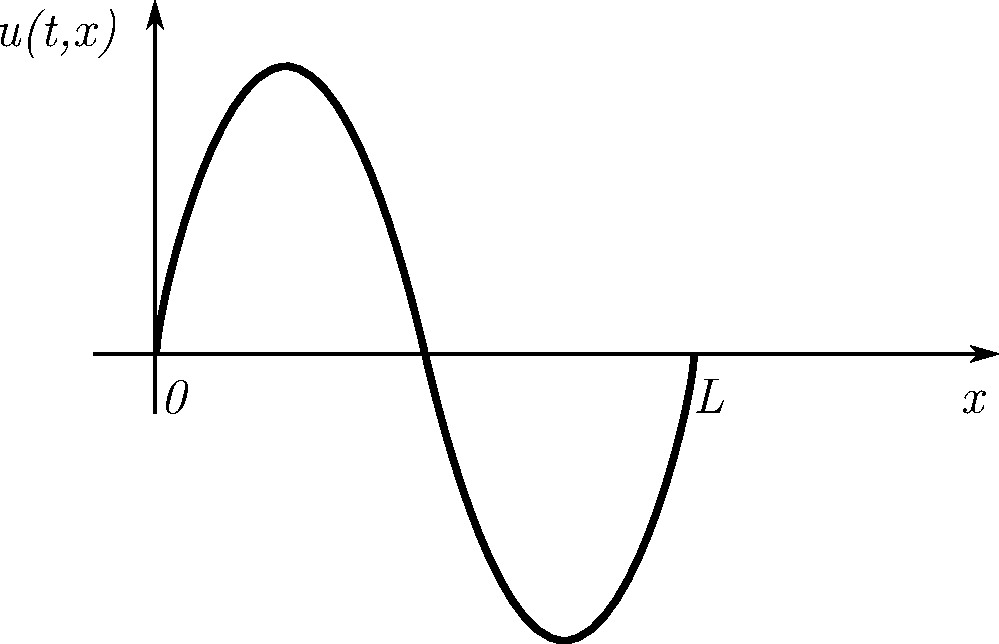
\includegraphics[width=0.6\textwidth]{wave_plane.pdf}
	\caption{$u(t,x)$ con $t$ fissato.}
	\label{wave_plane}
\end{figure}
\noindent
La conservazione della massa si scrive
\[
	\rho ds= \rho_0 dx
\]
quindi
\[
	\rho \sqrt{1 + u_x^2}= \rho_0
\]
Ora imponiamo che le componenti orizzontali delle forze si bilancino, dato lo
spostamento solo verticale.
Assumiamo che l'unica forza non completamente verticale  applicata nei punti
della corda, sia la tensione, forza diretta tangenzialmente data la corda
perfettamente
flessibile.
Precisamente, il vettore tensione ${\bf T}(t,x)$ indica la forza che la porzione
di corda a distanza dal punto $(x, u(t,x))$ esercita sulla porzione a sinistra.
Evidentemente ${\bf -T}(t,x)$ \`e la forza che la porzione a sinistra esercita
su
quella a destra.
\begin{figure}[H]
	\centering
	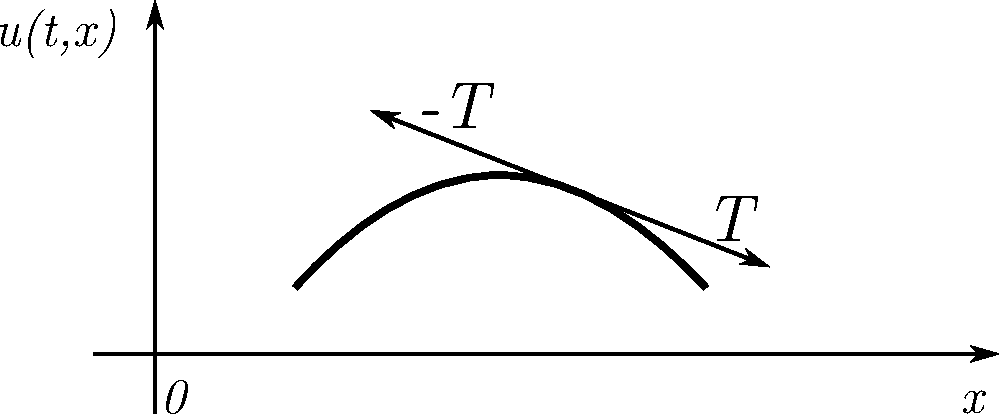
\includegraphics[width=0.6\textwidth]{tension.pdf}
	\caption{Tensione sulla corda.}
	\label{tension}
\end{figure}
\noindent
Indichiamo con $T(t,x)$ l'intensit\`a di ${\bf T}(t,x)$ e con $\alpha= \alpha
(t,x)$
l'inclinazione della corda rispetto alla posizione di riposo (asse $x$).
\[
	tg \alpha = u_x
\]
\begin{figure}[H]
	\centering
	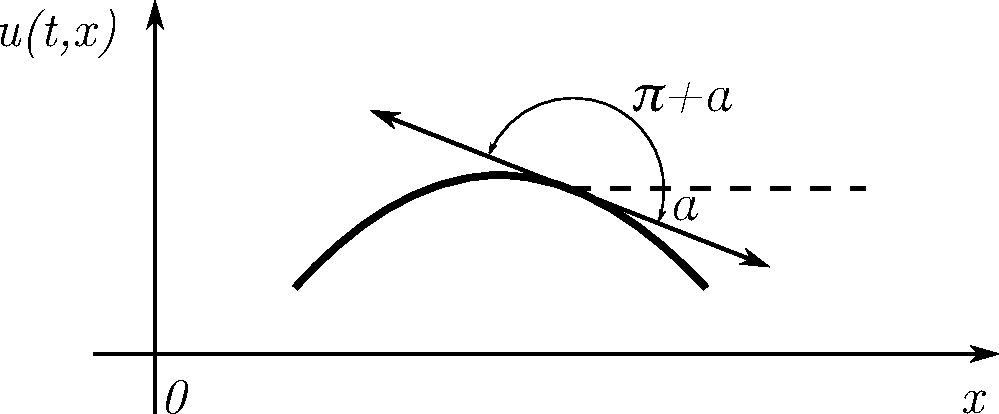
\includegraphics[width=0.6\textwidth]{tension_alpha.pdf}
	\caption{Tensione sulla corda con $\alpha$ mostrato.}
	\label{tension_alpha}
\end{figure}
\noindent
Il bilancio della componente orizzontale della tensione in un breve intervallo
$[x,x+\Delta x]$ impone
\[
	cos(\alpha + \pi)= - cos \alpha
\]
\begin{figure}[H]
	\centering
	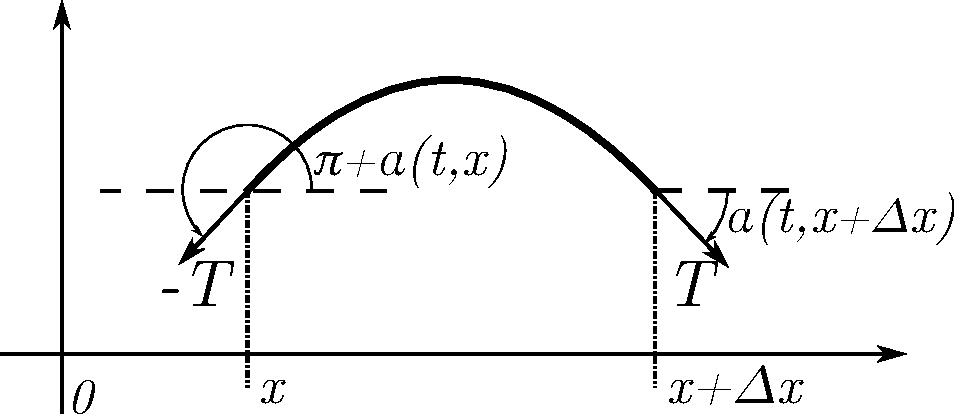
\includegraphics[width=0.8\textwidth]{tension_dx.pdf}
	\caption{Tensione sulla corda tra due punti distanti $dx$.}
	\label{tension_dx}
\end{figure}
\[
	T(t, x + \Delta x) cos \; \alpha(t, x + \Delta x)-
	T(t,x)cos \; \alpha(t,x)=0
\]
Dividendo per $\Delta x$ e mandando $\Delta x \to 0$
\[
	\frac{\partial}{\partial x}[T(t,x) cos \; \alpha(t,x)]=0
\]
da cui
\[
	T(t,x) cos \; \alpha(t,x)= \tau
\]
con $\tau$ indipendente da $x$.
La componente orizzontale della tensione, detta trazione, non dipende dalla
posizione. Se assumiamo che la tensione sia di intensit\`a proporzionale
alla lunghezza della porzione di corda che la esercita, allora $\tau$ \`e
indipendente anche da $t$ visto che la lunghezza in orizzontale \`e costante
$L$.\\
Calcoliamo ora la componente verticale della tensione nel tratto di corda
corrispondente a $[x, x+ \Delta x]$. Tenendo conto di $sin(\alpha + \pi)= - sin
\alpha$ e di $T= \tau/cos\alpha$, essa vale
\[
	T(t,x+\Delta x)sin \, \alpha(t, x+ \Delta x) - T(t,x)sin \, \alpha
(t,x)=
\]
\[
	\tau[tg \, \alpha (t, x + \Delta x)- tg  \, \alpha(t,x)]=
\]
\[
	\tau[u_x \, \alpha (t, x + \Delta x)- u_x \alpha(t,x)]=
	\tau \int_x^{x+\Delta x} u_{xx}(t,y) dy
\]
Essendo una trazione, essa corrisponde ad una forza.\\
Denotiamo ora con $f(t,x)$ gli eventuali carichi totali per unit\`a di massa; se
il
peso non \`e trascurabile $f(t,x)= -g + F(t,x)$, dove $g$ \`e l'accelerazione
di gravit\`a ed $F$ corrisponde ad altri ulteriori carichi. Quindi
\[
	=\tau \int_x^{x+\Delta x} u_{xx}(t,y) dy +
	\int_x^{x+\Delta x} f(t,y) \rho (t,y) \sqrt{1+ u_x^2(t,y)} dy
\]
Per il principio fondamentale della dinamica, forza = massa $\cdot$
accelerazione rappresenta sempre una forza
\[
	\underbrace{\int_x^{x+\Delta x} u_{tt}(t,y) \rho (t,y) \sqrt{1+
u_x^2(t,y)} dy}_{
	\text{accelerazione $\cdot$ massa}}
\]
perci\`o
\begin{align*}
	\int_x^{x+\Delta x} u_{tt}(t,y) \rho (t,y) \sqrt{1+ u_x^2(t,y)} dy&= \\
	\tau \int_x^{x+\Delta x} u_{xx}(t,y) dy &+
	\int_x^{x+\Delta x} f(t,y) \rho (t,y) \sqrt{1+ u_x^2(t,y)} dy
\end{align*}
che pu\`o essere scritta
\[
	\int_x^{x+\Delta x}\rho_0 u_{tt}(t,y)  dy=
	\int_x^{x+\Delta x} \tau u_{xx}(t,y) dy +
	\int_x^{x+\Delta x} \rho_0 f(t,y)  dy
\]
\[
	\int_x^{x+\Delta x} \left[
	\rho_0 u_{tt} - \tau u_{xx}-  \rho_0 f
	\right]dy= 0
\]
Per l'arbitrariet\`a del tratto $[x, x+ \Delta x]$, deve essere
\[
	\rho_0 u_{tt} - \tau u_{xx}-  \rho_0 f =0
\]
Dividendo per $\rho_0$ ed indicando $c^2=\tau / \rho_0$ si ha l'equazione
\[
	u_{tt} - c^2 u_{xx} = f
\]
dove la costante $c$ ha la dimensione di una velocit\`a.
\section{Problemi ben posti con lunghezza finita}
Esistenza, unicit\`a e dipendenza continua dai dati si hanno imponendo le
condizioni iniziali
\[
\begin{array}{ll}
	u(0,x)=g(x) & \text{(spostamento iniziale)}\\
	u_t(0,x)=h(x) & \text{(velocit\`a iniziale)}
\end{array}
\]
e selezionando uno tra i seguenti tipi di condizioni agli estremi.
\subsubsection{Dirichlet}
\[
	u(t,0)=a(t), \;\;\; u(t,L)=b(t)
\]
Si prescrive lo spostamento agli estremi.
In particolare gli estremi sono fissati per $a(t)= b(t)=0$
\subsubsection{Neumann}
\[
	\tau u_x(t,0)=a(t), \;\;\; -\tau u_c (t,L)=b(t)
\]
Si prescrive la componente verticale della tensione agli estremi.
\subsection{Energia}
L'energia immagazzinata dalla corda \`e data dalla somma dell'energia cinetica
e dell'energia potenziale. L'energia cinetica, dato
\[
	dL=Fdx=madx=m\frac{dv}{dt}dx=mdv\frac{dx}{dt}=mvdv
	\follows
	\int_0^t dL= m \int_0^t vdv
\]
\[
	L=\frac{1}{2}mv^2
\]
perci\`o
\[
	E_{cin}(t)= \frac{1}{2}\int_0^L \rho_0 u^2_t(t,x)dx
\]
L'energia potenziale vale il lavoro della trazione.
Calcoliamo l'allungamento per un tratto di corda $\Delta x$ a riposo. Vale
\[
	\int_x^{x + \Delta x} \sqrt{1+ u^2_x} dy - \Delta x=
	\int_x^{x + \Delta x} \left( \sqrt{1+ u^2_x}-1 \right) dy
\]
L'approssimazione lineare di $\sqrt{1+y}-1$ \`e $\frac{1}{2}y$ per $y \to 0$,
quindi l'approssimazione al primo ordine dell'allungamento \`e
\[
	\frac{1}{2} u^2_x \Delta x
\]
e l'energia potenziale vale
\[
	E_{pot}(t)= \frac{1}{2} \int_0^L \tau u^2_x (t,x)dx
\]
mentre l'energia totale \`e data da
\[
	E(t)= \frac{1}{2}\int_0^L \left[
	\rho_0 u^2_t + \tau u_x^2
	\right] dx
\]
Calcoliamo la variazione dell'energia:
\[
	E'(t)= \int_0^L \left[
	\rho_0 u_t u_{tt} + \tau u_x u_{xt}
	\right] dx
\]
Integriamo per parti il termine corrispondente all'energia potenziale
\[
	\int_0^L u_x u_{tx}dx=
	\left[ u_x u_t \right]_0^L -
	\int_0^L u_t u_{xx} dx
\]
avendo considerato continue le derivate e quindi lecito applicare il
teorema di Schwartz per invertire l'ordine di integrazione. Quindi
\[
	\int_0^L u_x u_{tx}dx=
	\tau \underbracket{\left[ u_x(t,L) u_t(t,L) -  u_x(t,0) u_t(t,0)
\right]}_{
	G(t)} -
	\int_0^L u_t u_{xx} dx
\]
Dunque
\[
	E'(t)= \int_0^L u_t (\rho_0 u_{tt} - \tau u_{xx})dx + \tau G(t)
\]
\[
	= \int_0^L u_t f dx + \tau G(t)
\]
tenuto conto dell'equazione $\rho_0 u_{tt} - \tau u_{xx}= f$.\\
In particolare, per $f=0$ (assenza di carichi) e per $G=0$ si ha $E'(t)=0$
da cui
\[
	E(t)= \text{costante}
\]
cio\`e l'energia \`e conservata.\\
$G=0$ si realizza con gli estremi fissati
\[
	u(t,0)=u(t,L)=0
\]
in quanto
\[
	u_t(t,0)=u_t(t,L)=0
\]
o con tensione verticale nulla agli estremi
\[
	u_x(t,0)=u_x(t,L)=0
\]
L'energia conservata \`e quella iniziale
\[
	E(t)=E(0)=\frac{1}{2}\int_0^L
	\left[
	\rho_0 u_t^2 (0,x) + \tau u^2_x (0,x)
	\right]dx
\]
\[
	=\frac{1}{2}\int_0^L
	\left[
	\rho_0 h^2(x) + \tau g'\,^2(x)
	\right]dx
\]
\subsection{Unicit\`a tramite l'energia}
Siano $u_1$, $u_2$ due soluzioni del problema di Dirichlet
\[
	\left\{
	\begin{array}{l}
		u_{tt} - c^2 u_{xx}= f \\
		u(0,x)=g(x) \\
		u_t(0,x)= h(x)\\
		u(t,0)=a(t), \;\;\; u(t,L)=b(t)
	\end{array}
	\right.
\]
la differenza $w=u_1-u_2$ risolve il problema
\[
	\left\{
	\begin{array}{l}
		w_{tt} - c^2 w_{xx}= f \\
		w(0,x)=0 \\
		w_t(0,x)= 0\\
		w(t,0)=0, \;\;\; w(t,L)=0
	\end{array}
	\right.
\]
L'equazione per $w$ \`e omogenea con dati di Dirichlet nulli, quindi l'energia
si conserva e vale per ogni $t\geq 0$ l'energia iniziale.
Poich\'e i dati iniziali sono anch'essi nulli, l'energia iniziale \`e nulla.
In definitiva $E(t)=0$ cio\`e
\[
	\int_0^L [\rho_0 w^2_t + \tau w_x^2]=0
\]
da cui $w_t=0$ e $w_x=0$.\\
La funzione $w(t,x)$ \`e quindi costante in $(t,x)$, ed essendo $w=0$ per
$t=0$, si ha
\[
	w(t,x)=0 \;\;\; \text{per ogni }(t,x)
\]
Il problema di Dirichlet ha soluzione unica.\\
Stesse considerazioni per il problema di Neumann.
\subsection{Esistenza e regolarit\`a della soluzione}
Consideriamo la vibrazione di una corda fissata agli estremi e senza carichi
\[
	\left\{
	\begin{array}{l}
		u_{tt} - c^2 u_{xx}= 0 \\
		u(0,x)=g(x) \\
		u_t(0,x)= h(x)\\
		u(t,0)=0, \;\;\; u(t,L)=0
	\end{array}
	\right.
\]
Cominciamo nel cercare soluzioni di
\[
	\left\{
	\begin{array}{l}
		u_{tt} - c^2 u_{xx}= 0 \\
		u(t,0)=0, \;\;\; u(t,L)=0
	\end{array}
	\right.
\]
con il metodo della separazione delle variabili imponendo
\[
	u(t,x)=v(t)w(x)
\]
\[
	w(0)=w(L)=0
\]
si ha
\[
	v''(t)w(x)=c^2w''(x)v(t)
\]
da cui
\[
	\frac{1}{c^2} \frac{v''(t)}{v(t)}= \frac{w''(x)}{w(x)}
\]
che si pu\`o realizzare solo con
\[
	\frac{1}{c^2} \frac{v''(t)}{v(t)}= k = \frac{w''(x)}{w(x)}
\]
con $k$ costante.\\
Consideriamo il problema
\[
	\left\{
	\begin{array}{l}
		w''= kw \\
		w(0)=0, \;\;\; w(L)=0
	\end{array}
	\right.
\]
Si hanno soluzioni non banali solo per $k= -\mu <0$
perch\'e per $k>0$ o $k=0$ le condizioni agli estremi portano a $w=0$,
essendo in tali casi
\[
	w=ae^{x\sqrt{k}} + b e^{-x \sqrt{k}} \;\;\; \text{o} \;\;\;
	w=ax+b
\]
il rispettivo integrale generale. In entrambi i casi
\[
	\begin{cases}
		w(0)=0 \\
		w(L)=0
	\end{cases}
	\follows
	\begin{cases}
		a=0 \\
		b=0
	\end{cases}
\]
Sia dunque $k=-\mu < 0$ che porta
\[
	w=a \, cos(\mu x) + b \, sin (\mu x)
\]
\[
	\begin{cases}
		w(0)=0 \\
		w(L)=0
	\end{cases}
	\follows
	\begin{cases}
		a=0 \\
		b \, sin (\mu L)=0
	\end{cases}
\]
Abbiamo soluzioni non nulle per
\[
	\mu= \mu_m = \frac{m \pi}{L} \;\;\; m=1,2,3, \ldots
\]
date da
\[
	w_m= b_m sin \left( \frac{m\pi}{L} x \right)
\]
Veniamo all'equazione
\[
	v''(t)= -\mu^2 t^2 v(t)
\]
per il fattore dipendente da $t$.
Le soluzioni sono date da
\[
	v= a \, cos(\mu c t) + b \, sin (\mu c t)
\]
Abbiamo cos\`i trovato le infinite soluzioni di
\[
	\left\{
	\begin{array}{l}
		u_{tt} - c^2 u_{xx}= 0 \\
		u(t,0)=0, \;\;\; u(t,L)=0
	\end{array}
	\right.
\]
date da
\[
	u_m=
	\underbrace{\left[ a_m \, cos \left( \mu c t \right)
	+ b_m \, sin \left( \mu c t \right) \right]}_{A_m(t)}
	sin \left( \frac{m\pi}{L} x \right)
\]
\[
	u_m=
	\left[ a_m \, cos \left( \frac{mc\pi}{L} t \right)
	+ b_m \, sin \left( \frac{mc\pi}{L} t \right) \right]
	 sin \left( \frac{m\pi}{L} x \right)
\]
con $m=1,2,3, \ldots$\\
Queste sono dette le ``vibrazioni possibili '' della corda fissata agli estremi.
La forma della vibrazione \`e prescritta dalla funzione $sin \left(
\frac{m\pi}{L} x \right)$
con ampiezza $A_m(t)$ di segno ed intensit\`a variabile nel tempo, ma periodica
di periodo minimo
\[
	T_m= 2\pi \frac{L}{mc \pi}= \frac{2L}{mc}
\]
e la relativa frequenza
\[
	\frac{1}{T_m}= m\frac{c}{2L}
\]
\begin{figure}[t]
	\centering
	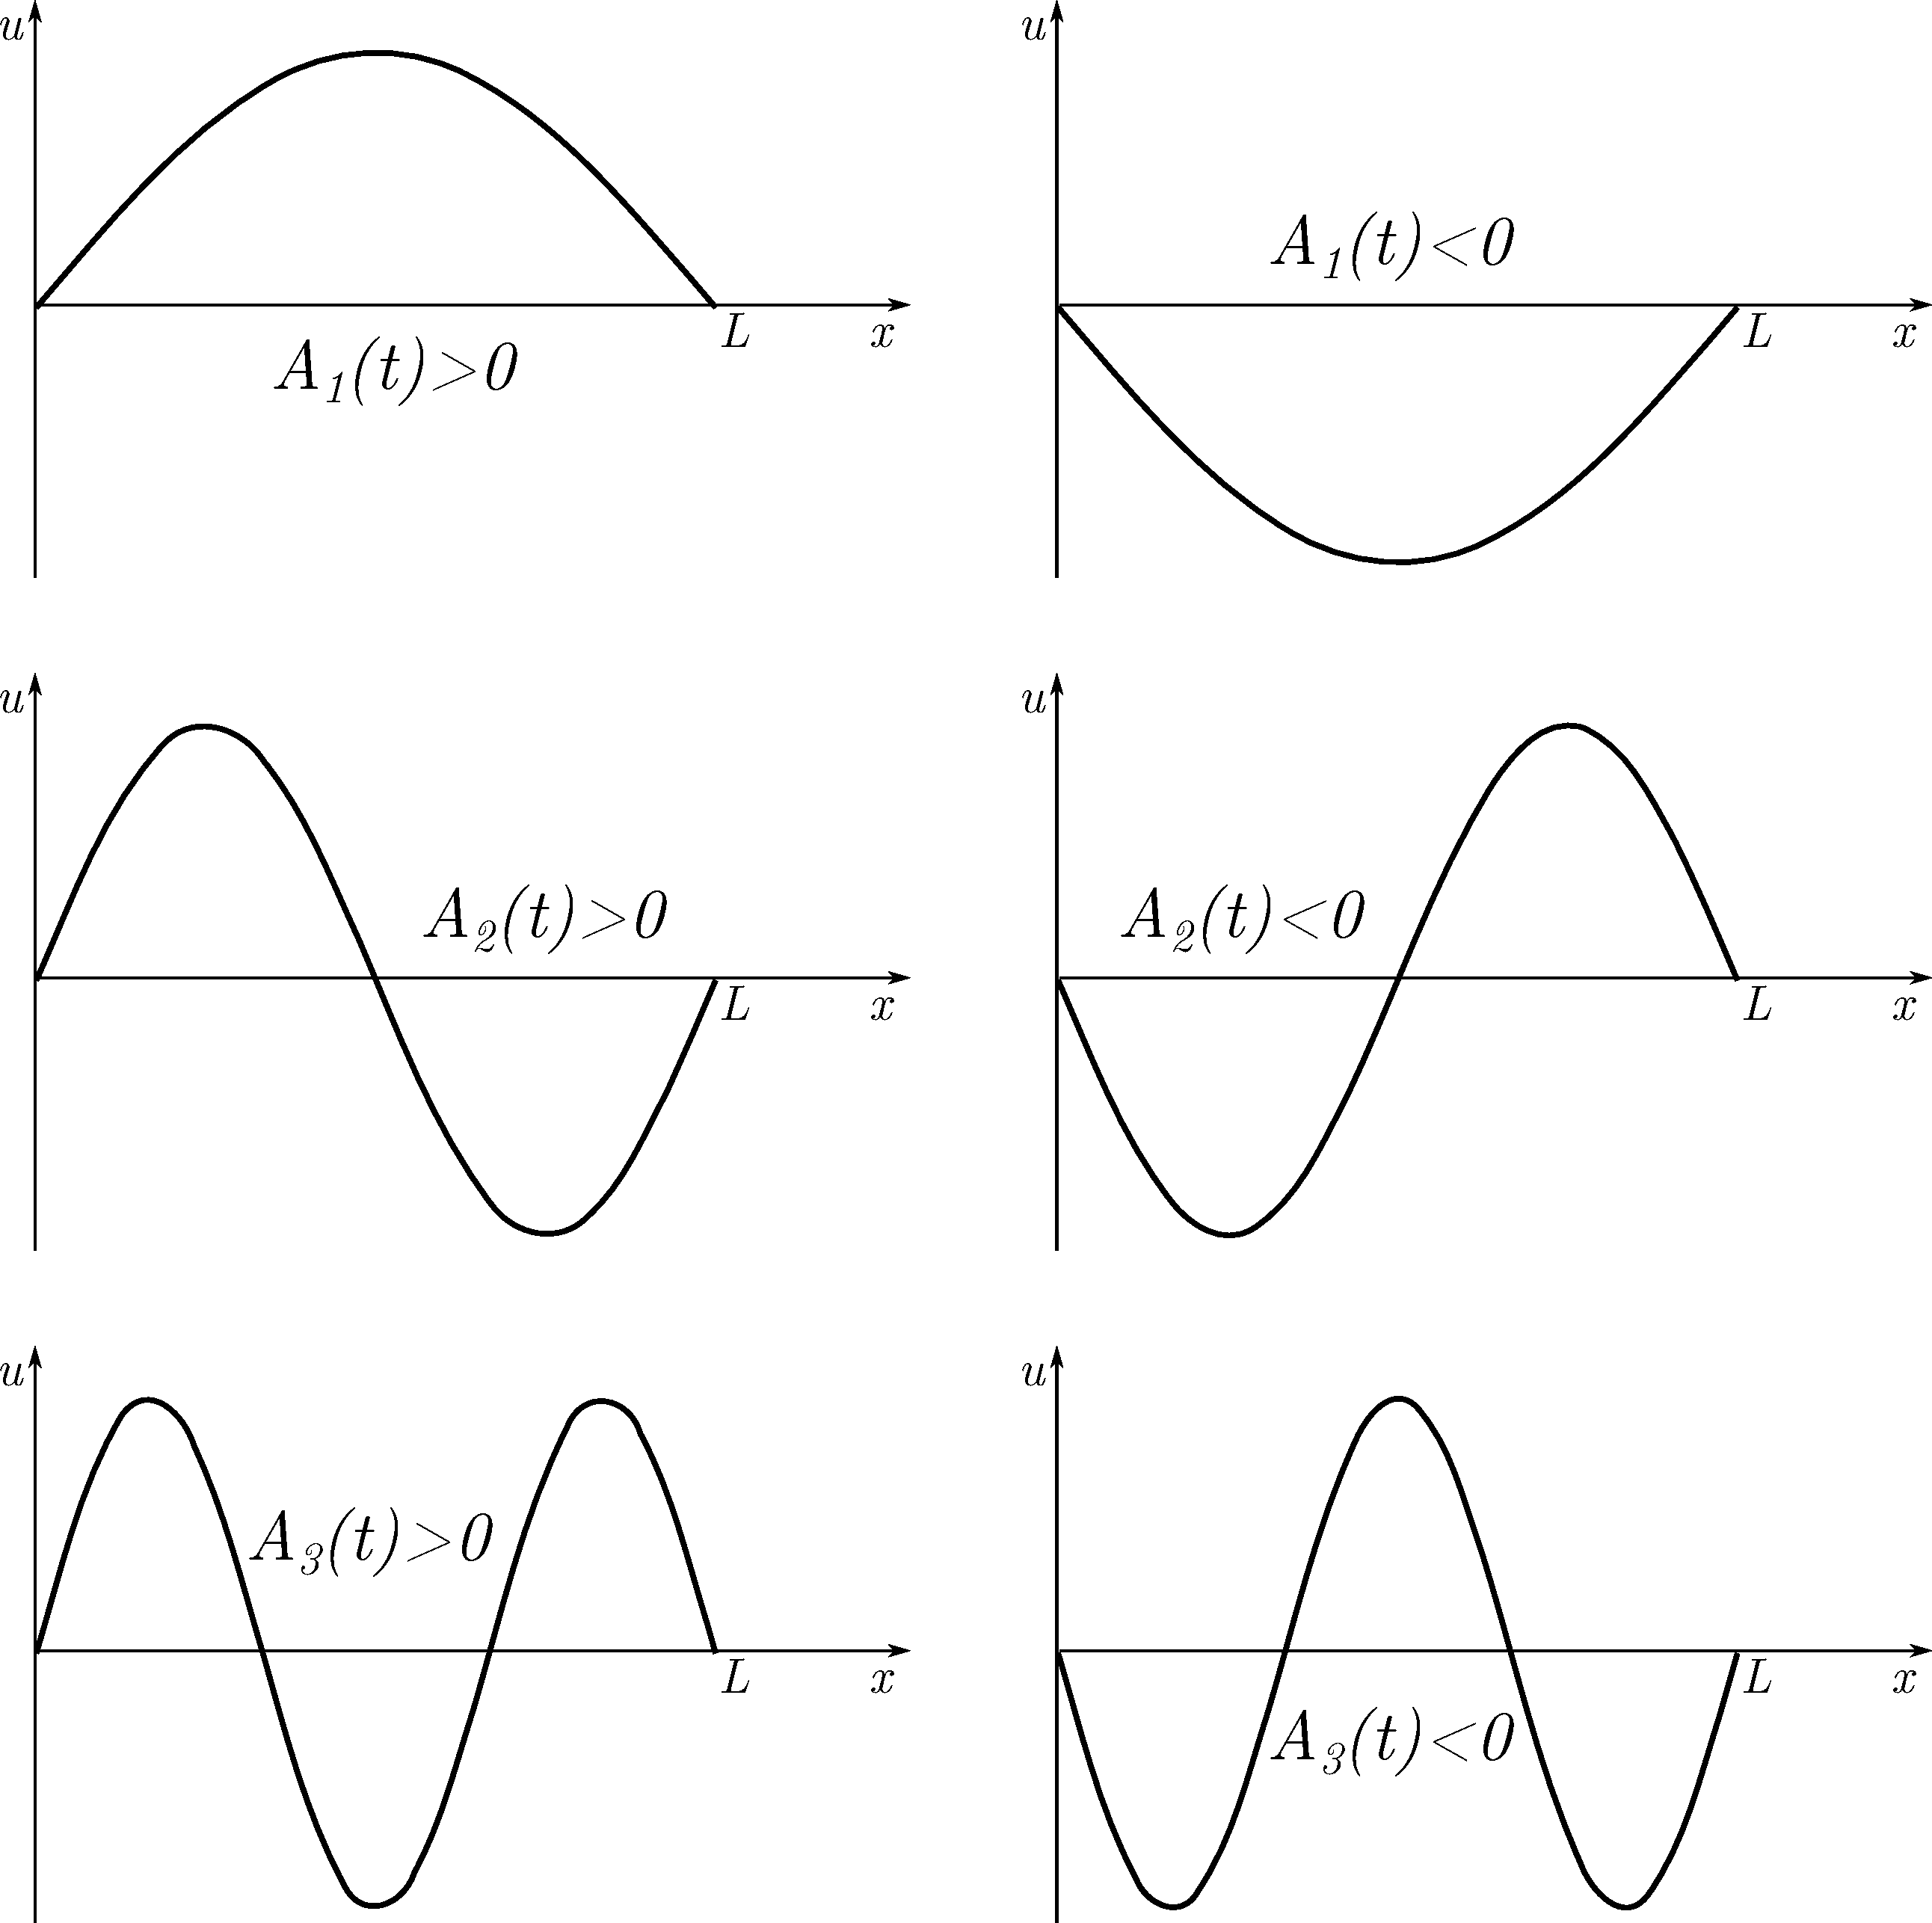
\includegraphics[width=\textwidth]{wave_modes.pdf}
	\caption{Alcune ``istantanee'' delle prime tre vibrazioni possibili a
$t$ fissato.}
	\label{wave_modes}
\end{figure}
\noindent
Come si pu\`o notare in fig. \ref{wave_modes}, dopo un tempo $T=\frac{2L}{c}$
si rivedono le stesse configurazioni: per $u_1$ \`e la priva volta, per $u_2$ la
seconda e per $u_3$ la terza volta che si osserva lo stesso grafico.\\
La sovrapposizione di vibrazioni con frequenza tutte multiple della stessa
frequenza di base
\[
	\frac{1}{T_1}= \frac{c}{2L}
\]
produce il suono armonioso della corda vibrante. La sovrapposizione
\[
	u= \sum_{m=1}^{\infty} u_m =
	\sum_{m=1}^{\infty} \left[ a_m \, cos \left( \frac{mc\pi}{L} t \right)
	+ b_m \, sin \left( \frac{mc\pi}{L} t \right) \right]
	 sin \left( \frac{m\pi}{L} x \right)
\]
\`e la soluzione completa.\\
Si definiscono quindi le condizioni iniziali
\[
	\begin{array}{l}
	u(0,x)= g(x)
 	\\
	u_t(0,x)= h(x)
	\end{array}
\]
Ponendo $t=0$ nell'espressione di $u$ e $u_t$
\[
	g(x)= \sum_{m=1}^{\infty} a_m \, sin \left( \frac{m\pi}{L} x \right)
\]
e
\[
	h(x)= \sum_{m=1}^{\infty} \frac{mc\pi}{L} b_m \, sin \left(
	\frac{m\pi}{L} x \right)
\]
Si sviluppano i dati $g(x)$ e $h(x)$ in serie di sole sinusoidi per $x \in
[0,L]$ effettuando il prolungamento continuo dispari all'intervallo $[-L,L]$.\\
I coefficienti sono quindi forniti da
\[
	a_m= \frac{2}{L} \int_0^L g(x) sin \left( \frac{m\pi}{L} x \right) dx
\]
\[
	b_m= \frac{2}{mc \pi} \int_0^L h(x) sin \left( \frac{m\pi}{L} x \right)
dx
\]
La funzione $u(t,x)$ cos\`i trovata risolve il problema almeno nel senso delle
distribuzioni.
Affinch\'e sia una soluzione in senso usuale occorre che si possa derivare due
volte in $dt$ ed in $dx$ sotto il segno di serie.
Questo \`e possibile se se i coefficienti $a_m$ e $b_m$ decadono almeno come
$\/m^4$: derivando due volte si producono addendi con coefficienti $m^a_m$,
$m^2b_m$. La condizione
\[
	m^2|a_m|\leq \frac{cost.}{m^2}, \;\;\; m^2|b_m|\leq \frac{cost.}{m^2}
\]
\`e sufficiente per garantire poi la convergenza dominata della serie ottenuta
derivando termine a termine.\\
La regolarit\`a $C^4$ per $g$ e $C^3$ per $h$ ($b_m$ ha gi\`a un $m$ a
denominatore) \`e una ipotesi sufficiente.\\
Osserviamo una diversit\`a fondamentale con l'equazione della diffusione. Per
questa ultima, qualunque sia la regolarit\`a del dato iniziale, i coefficienti
di Fourier della soluzione per $t>0$ decadono come $e^{-m^2 \pi^2 Dt/L}$ cio\`e
come $e^{-\alpha m^2}$ per $m \to +\infty$.
La soluzione ha in quel caso tutte le derivate in $dt$ e in $dx$ per $t>0$.
\`E questo l'effetto regolarizzante della diffusione, assente per l'equazione
della corda vibrante. Ora la soluzione \`e $C^k$ se i dati sono $g \in C^{k+2}$
e $h \in C^{k+1}$, $k\geq 2$. La regolarit\`a dei dati fornisce la regolarit\`a
della soluzione.\\
Non abbiamo ora soluzioni stazionare n\'e regime transitorio. In assenza di
attrito, la corda vibra all'infinito con una sovrapposizione di vibrazioni
periodiche stabilite dai dati iniziali.
\subsection{Dipendenza continua dai dati}
Indichiamo con $||u(t, \cdot)||_2$ la norma in $L^2$ della soluzione al tempo
$t$ fissato
\[
	||u(t, \cdot)||_2=
	\left(
	\int_0^L |u(t,x)|^2 dx
	\right)^{1/2}
\]
Per Parseval, dallo sviluppo di Fourier
\[
	u(t,x)= \sum_{m=1}^{\infty} \left[ a_m \, cos \left( \frac{mc\pi}{L} t
\right)
	+ b_m \, sin \left( \frac{mc\pi}{L} t \right) \right]
	 sin \left( \frac{m\pi}{L} x \right)
\]
segue
\[
	||u(t, \cdot)||_2^2 = \sum_{m=1}^{\infty} \left[ a_m \, cos \left(
	\frac{mc\pi}{L} t \right)
	+ b_m \, sin \left( \frac{mc\pi}{L} t \right) \right]^2
\]
usando $|cos \alpha |\leq 1$, $|sin \alpha |\leq 1$, $2ab \leq a^2 + b^2$
\[
	=\sum_{m=1}^{\infty} \left[ a_m \,
	+ b_m \, \right]^2 =
	\sum_{m=1}^{\infty} \left[ a_m^2 + b_m^2 + 2ab \right]
	\leq 2 \sum_{m=1}^{\infty} \left[ a_m^2 + b_m^2 \right]
\]
Sempre per Parseval
\[
	\sum_{m=1}^{\infty} a_m^2 =
	\int_0^L |g(x)|^2 dx = ||g||_2^2
\]
In quanto gli $a_m$ sono esattamente i coefficienti di Fourier di $g(x)$. I
$b_m$ sono i coefficienti di $h(x)$ divisi per $\frac{mc \pi}{L}\leq
\frac{c \pi}{L}$, quindi
\[
	\sum_{m=1}^{\infty} b_m^2 \leq \frac{L^2}{c^2 \pi^2}||h||^2_2
\]
Riassumendo
\[
	||u(t,\cdot)||_2^2 \leq M(||g||_2^2 + ||h||_2^2)
\]
Per linearit\`a, se $u_1$ e $u_2$ sono soluzioni del problema con dati di
Cauchy ($g_1,h_1$) e ($g_2,h_2$) rispettivamente, allora
\[
	||u_1(t,\cdot) - u_2(t,\cdot)||_2^2 \leq M(||g_1 - g_2||_2^2 + ||h_1 -
	h_2||_2^2)
\]
che esprime la dipendenza continua dai dati nel problema di Cauchy-Dirichlet
con dati di Dirichlet nulli.
\section{Il problema di Cauchy globale}
\subsection{Formula di D'Alambert}
Consideriamo il problema di Cauchy globale (L=$\infty$)
\[
	\begin{cases}
		u_{tt} - c^2 u_{xx}= 0 , \;\;\;\; t>0, \;\; x \in \mathbb{R} \\
		u(0,x)= g(x)\\
		u_t (0,x)= h(x)
	\end{cases}
\]
L'equazione
\[
	\left( \partial_t^2 -c^2 \partial_x^2 \right) u=0
\]
si scrive
\[
	\left( \partial_t -c \partial_x \right)\left( \partial_t + c
	\partial_x \right) u=0
\]
Posto
\[
	u(t,x)= v(y,\eta)
\]
con
\[
	y=x -ct, \;\;\; \eta= c+ ct
\]
si ha
\[
	\partial_tu= -c \partial_y v + c\partial_\eta v
\]
\[
	\partial_xu= \partial_y v + \partial_\eta v
\]
cio\`e
\[
	\partial_t - c \partial_x = -2c \partial_y
\]
\[
	\partial_t + c\partial_x = 2c \partial_n
\]
Abbiamo
\[
	u_{tt}- c^2u_{xx}= \underbrace{\left( \partial_t -c \partial_x
	\right)}_{-2c \partial_y}
	\underbrace{\left( \partial_t + c
	\partial_x \right)}_{2c \partial_\eta} u= -4c \, \partial_{y}
	\partial_{\eta} v=0
	\follows v_{yn}=0
\]
e l'equazione $v_{yn}=0$ ha per integrale generale
\[
	\frac{\partial}{\partial \eta} \left(
	\frac{\partial}{\partial y} v \right)=0
\]
\[
	\frac{\partial}{\partial \eta} v (y, \eta)=0
\]
\[
	v(y, \eta)= \int f(\eta) d\eta + \underbrace{ G(y) }_{\mathclap{
	\text{Costante rispetto a }\eta}}
\]
\[
	v(y, \eta)= F(\eta)+ G(y)
\]
con $F$, $G$ arbitrarie funzioni derivabili.\\
Tornando alle variabili iniziali
\[
	u(t,x)=F(x+ct)+G(x-ct)
\]
cio\`e $u$ \`e la sovrapposizione di due onde viaggianti (solitoni) in
direzioni opposte, alla medesima velocit\`a $c$.
\begin{figure}[H]
	\centering
	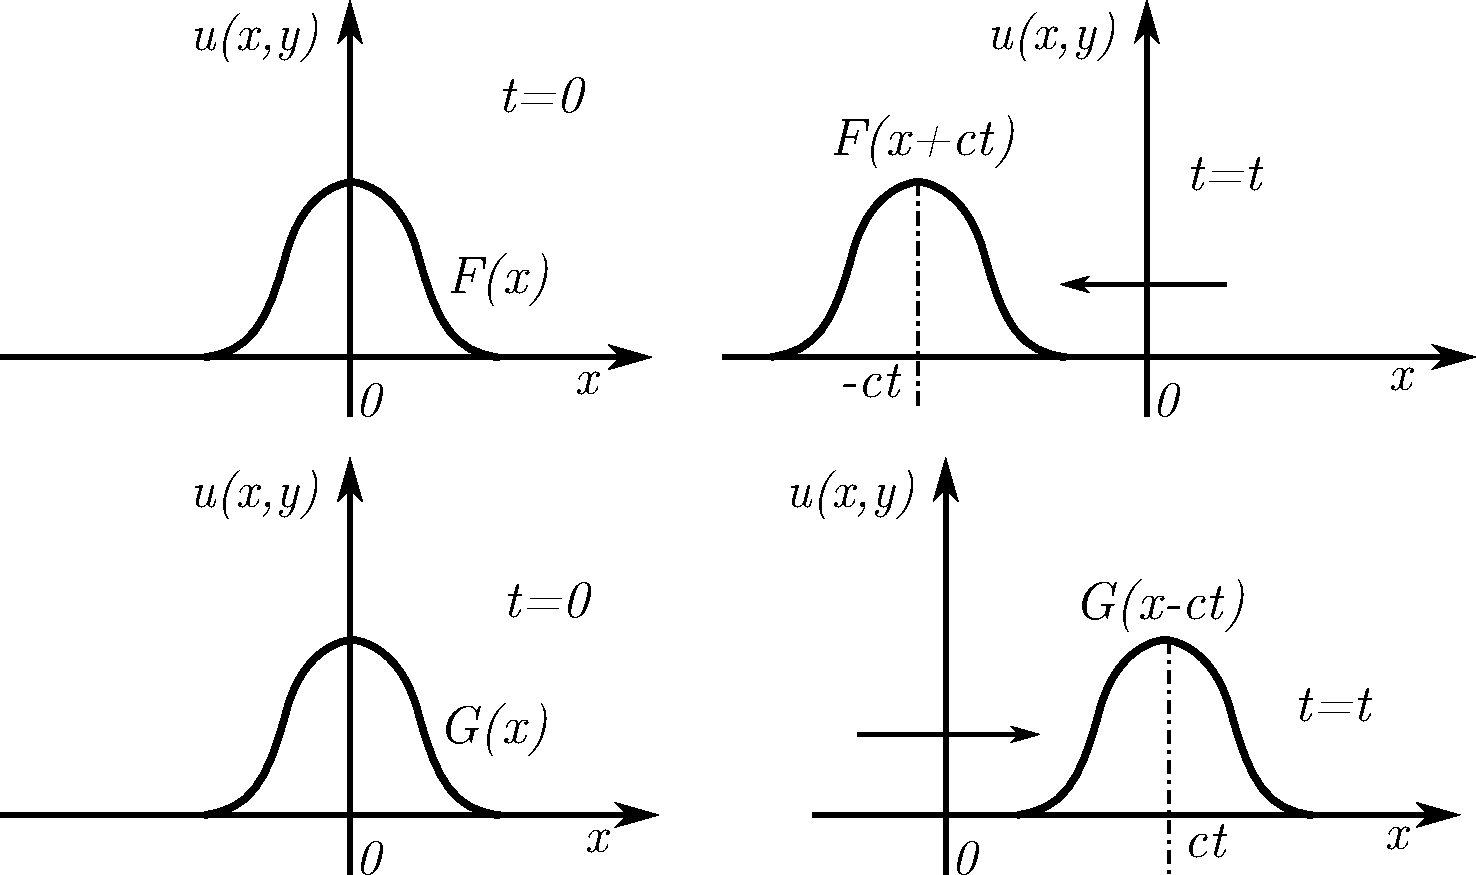
\includegraphics[width=\textwidth]{soliton.pdf}
	\caption{Onde viaggianti (solitoni).}
	\label{soliton}
\end{figure}
\noindent
Imponendo le condizioni iniziali
\[
	g(x)= u(0,x)= F(x)+ G(x)
\]
\[
	h(x)=u_t(0,x)=cF'(x)- cG'(x)
\]
(si \`e usato $u_t(t,x)= cF'(x+ct)- cG'(x+ct)$)
si ottiene
\[
	\left\{
	\begin{array}{ll}
		F+G= g\\
		cF-cG= H & H(x)= \int h(x)dx
	\end{array}
	\right.
\]
moltiplico la prima per $c$ e poi sommo o sottraggo; se sottraggo
\[
	2cG= cg - H
\]
se sommo
\[
	2cF= cg + H
\]
da cui
\[
	F=\frac{1}{2}g + \frac{1}{2c}H, \;\;\; G=\frac{1}{2}g-\frac{1}{2c}H
\]
ed infine
\[
	u(t,x)= \frac{1}{2}g(x+ct)+ \frac{1}{2}g(x-ct)+\frac{1}{2c}
	[H(x+ct)-H(x-ct)]
\]
\[
	= \frac{1}{2}g(x+ct)+ \frac{1}{2}g(x-ct)+\frac{1}{2c}
	\int_{x-ct}^{x+ct} h(y)dy
\]
Questa \`e nota come la formula di D'Alambert.\\
Definisce una soluzione di classe $C^2$ non appena $g \in C^2$ e $h \in C^1$.
Per come \`e stata ottenuta \`e l'unica soluzione di classe $C^2$ sotto tali
ipotesi di regolarit\`a dei dati.\\
Il metodo con cui \`e stata ottenuta mostra anche che $u$ \`e l'unica soluzione
di classe $C^k$ per dati $g \in C^k$, $h \in C^{k-1}$. Si noti l'assenza di
effetti regolarizzanti, la regolarit\`a dei dati stabilisce la regolarit\`a
della soluzione.\\
Dalla formula di D'Alambert si ottiene direttamente la dipendenza continua dai
dati secondo la norma di $L^{\infty}$
\[
	||f||_{\infty}= \sup_x|f(x)|
\]
Infatti
\[
	|u(t,x)| \leq \frac{1}{2}|g(x+ct)| + \frac{1}{2}|g(x-ct)|+
	\frac{1}{2c}\int_{x-ct}^{x+ct} |h(y)| dy
\]
\[
	\leq \frac{1}{2}||g||_\infty + \frac{1}{2}||g||_\infty+
	\frac{1}{2c}\int_{x-ct}^{x+ct} ||h||_\infty dy
\]
\[
	= ||g||_\infty + \frac{2ct}{2c}||h||_\infty= ||g||_\infty +
	t ||h||_\infty
\]
da cui
\[
	||u(t, \cdot)||_\infty \leq ||g||_\infty + t||h||_\infty
\]
Se ora $u_1$, $u_2$ sono soluzioni con rispettivi dati iniziali $(g_1,h_1)$ e
$(g_2,h_2)$, per linearit\`a abbiamo la stima di dipendenza continua dai dati.
\[
	||u_1(t, \cdot) - u_2(t, \cdot)||_\infty
	\leq ||g_1 -g_2||_\infty + t||h_1-h_2||_\infty
\]
Una ulteriore utile osservazione sulla formula di D'Alambert \`e che basta
saper risolvere il problema con $g=0$ ed $h$ arbitrario. Infatti la derivata in
$dt$ del termine corrispondente al dato $h$ vale
\[
	\frac{1}{2c}\partial_t \int_{x-ct}^{x+ct} h(y)dy=
	\frac{1}{2c}= [h(x+ct)c - h(x-ct)(-c)]=
\]
\[
	=\frac{1}{2} [h(x+ct) + h(x-ct)]
\]
che ha lo stesso aspetto del termine corrispondente al dato $g$. La formula di
D'Alambert diventa
\[
	u(t,x)= \frac{\partial}{\partial t}v_g(t,x)+ v_h(t,x)
\]
dove $v_H$ indica la soluzione del problema
\[
	\begin{cases}
		v_{tt}= c^2 v_{xx}\\
		v(0,x)= 0 \\
		v_t(0,x)= H(x)
	\end{cases}
\]
\subsection{Caratteristiche, Domini di dipendenza, Domini d influenza}
Nella rappresentazione
\[
	u(t,x)=F(x+ct) + G(x-ct)
\]
abbiamo il termine $F(x-ct)$ che \`e costante lungo la retta $\gamma^+$ di
equazione
\[
	x+ct=z, \;\;\; \text{$z$ fissato sull'asse $x$}
\]
nel piano $(x,t)$. Analogamente $G(x-ct)$ \`e costante lungo la retta
$\gamma^-$ di equazione
\[
	x-ct=z, \;\;\; \text{$z$ fissato sull'asse $x$}
\]
\begin{figure}[H]
	\centering
	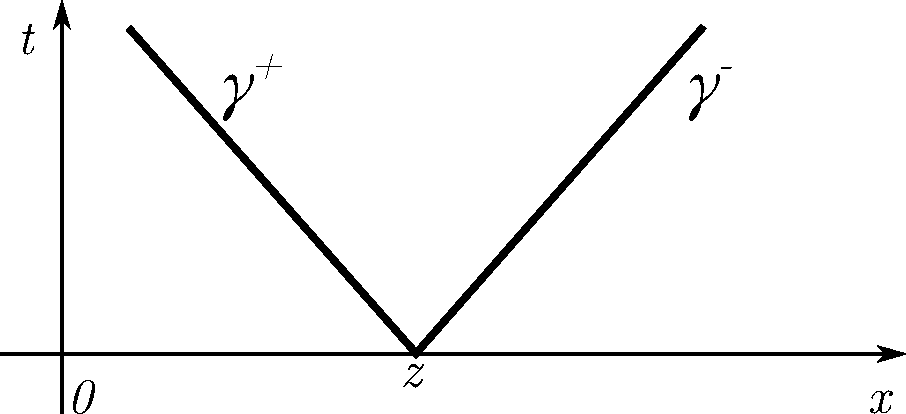
\includegraphics[width=0.6\textwidth]{char_rect.pdf}
	\caption{Rette caratteristiche.}
	\label{char_rect}
\end{figure}
\noindent
Queste rette che trasportano i dati iniziali si chiamano caratteristiche. Il
cono nel piano $(x,t)$ delimitato dalle caratteristiche per $(z,0)$ si chiama
dominio di influenza del punto $z$.
\begin{figure}[H]
	\centering
	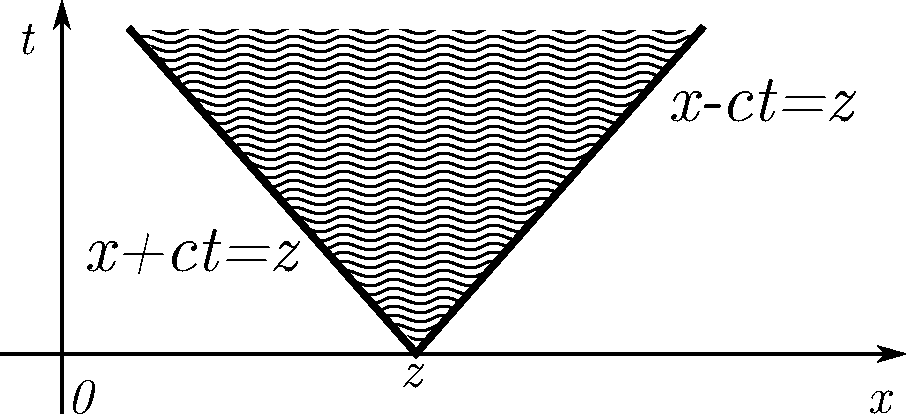
\includegraphics[width=0.6\textwidth]{infl_dom.pdf}
	\caption{Dominio di influenza.}
	\label{infl_dom}
\end{figure}
\noindent
I valori dei dati iniziali in $z$ influenzano i valori di $u(t,x)$ nei punti
del dominio cos\`i identificato. Una perturbazione iniziale localizzata in $z$
al tempo $t=0$, raggiunge il punto $x$ in un tempo
\[
	t=\frac{|x-z|}{c}
\]
In maniera simmetrica, la formula di D'Alambert dice che in un punto fissato
$(\bar{t}, \bar{x})$ il valore $u(\bar{t}, \bar{x})$ dipende solo dai valori
del dato iniziale $g(x)=u(0,x)$ nei due punti $\bar{x}+ c\bar{t}$ ed $\bar{x}-
c\bar{t}$ e dai valori del dato $h(x)=u_t(0,x)$ nell'intervallo $[\bar{x}-
c\bar{t}, \bar{x}+ c\bar{t}]$. Il valore $u(\bar{t}, \bar{x})$ dipende solo dai
valori di $g$, $h$ in $[\bar{x}- c\bar{t}, \bar{x}+ c\bar{t}]$.
Questo intervallo si chiama dominio di dipendenza e si ottiene tracciando le
caratteristiche per $(\bar{t}, \bar{x})$ fino ad incontrare l'asse $x$ nei
punti $\bar{x} - c\bar{t}$, $\bar{x}+ c\bar{t}$
\begin{figure}[H]
	\centering
	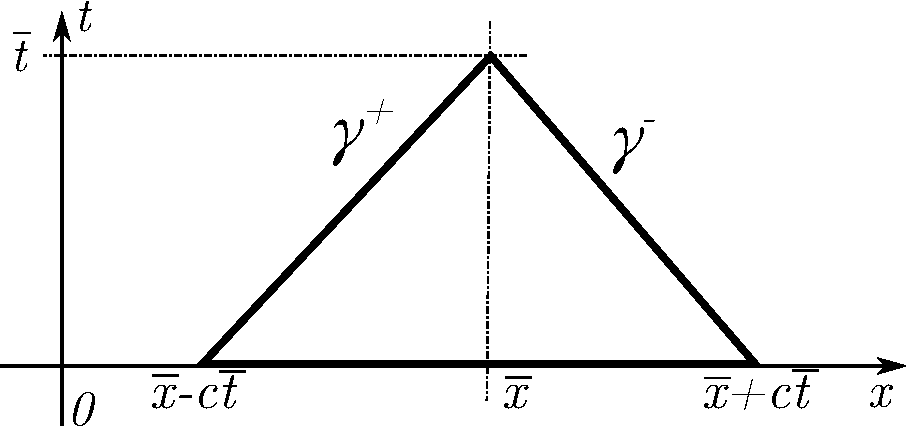
\includegraphics[width=0.6\textwidth]{dep_dom.pdf}
	\caption{Dominio di dipendenza.}
	\label{dep_dom}
\end{figure}
\noindent
Sempre da
\[
	u(t,x)= F(x+ct) + G(x-ct)
\]
si ottiene un'altra interessante propriet\`a.\\
Il rettangolo in fig. \ref{char_recta} si chiama rettangolo caratteristico.
\vspace{5mm}
\begin{figure}[H]
	\centering
	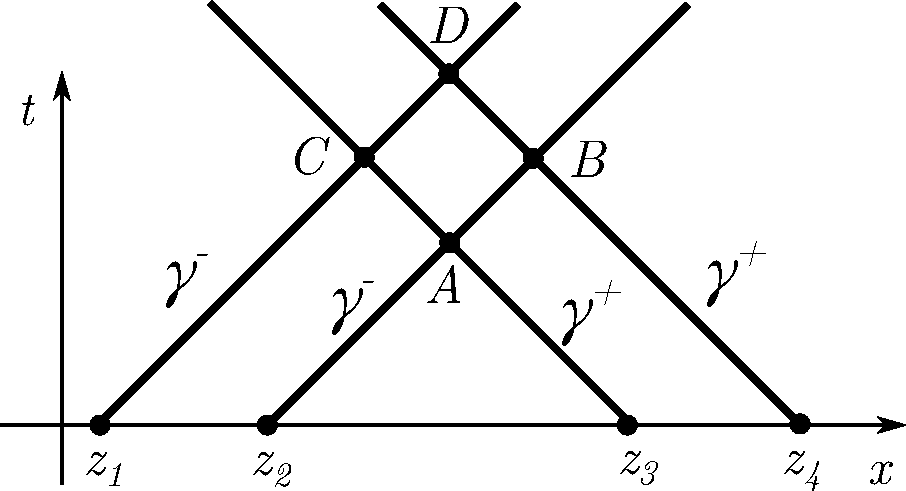
\includegraphics[width=0.6\textwidth]{char_recta.pdf}
	\caption{Rettangolo caratteristico.}
	\label{char_recta}
\end{figure}
\noindent
Abbiamo
\[
	\begin{array}{lcl}
		F(A)=F(C) 	&,&	F(D)=F(B)\\
		G(A)=G(B)	&,&	G(C)=G(D)
	\end{array}
\]
da cui
\[
	u(A)+u(D)=F(A)+F(G)+F(D)+G(D)
\]
coincide con
\[
	u(B)+u(C)= F(B)+G(B)+F(C)+G(C)
\]
Da
\[
	u(A)+u(D)=u(C)+u(B)
\]
segue che nota $u$ in tre vertici si trova $u$ nel quarto vertice.

\subsection{Conservazione dell'energia}
Si ricorda che l'energia \`e data da
\[
	E(t)=\frac{1}{2} \intR \left(
	\rho_0 u_t^2 + \tau u_x^2
	\right) dx
\]
Il teorema di Parseval afferma
\[
	\intR |f(x)|^2 dx =
	\frac{1}{2\pi}
	\intR |\hat{f}(\lambda)|^2d \lambda
\]
Perci\`o, dato $f=u_t \follows |\hat{f}|^2=|v_t|^2$ e
$f=u_x \follows |\hat{f}|^2=|i\lambda v|^2=\lambda^2|v|^2$
\[
	E(t)= \frac{1}{4 \pi} \intR
	\left(
	\rho_0 |v_t|^2 + \tau \lambda^2 |v|^2
	\right) d\lambda
\]
La derivata di $|g(t)|^2$ con $g(t)$ a valori complessi pu\`o essere ottenuta
considerando
\[
	|g(t)|^2= g(t)\underbracket{g^*(t)}_{\mathclap{\text{Coniugato}}}
\]
\[
	\frac{d}{dt}|g(t)|^2=
	g'(t) g^{*} (t) + g(t)(g^{*})'(t)= g'(t)g^{*}(t)+
	\left(
	g'(t)g^*(t)
	\right)^*
\]
\[
	=2 {\mathcal Re} \left\{ g'(t)g^*(t) \right\}
	=2 {\mathcal Re} \left\{ (g'(t)g^*(t))^* \right\}
	=2 {\mathcal Re} \left\{ (g'(t))^* g(t) \right\}
\]
Ora
\[
	E'(t)= \frac{1}{4\pi} \intR \left[
	\rho_0 \, 2 {\mathcal Re} \{v_t^* \, v_{tt}\}+
	\tau \lambda^2 \, 2 {\mathcal Re} \{ v \,v_t^* \}
	\right] d \lambda
\]
\[
	=\frac{1}{2\pi} \intR \left[
	{\mathcal Re} \{ \rho_0 v_t^* v_{tt} + \tau \lambda^2 vv_t^* \}
	\right] d \lambda
\]
\[
	=\frac{1}{2\pi} \intR \left[
	{\mathcal Re} \{ v_t^* (\rho_0 v_{tt} + \tau \lambda^2 v) \}
	\right] d \lambda
\]
Data $\rho_0 v_{tt} + \tau \lambda^2 v=0$ dalla trasformata di $\rho_0 u_{tt} -
\tau u_{xx}= 0$
\[
	=\frac{1}{2\pi} \intR \left[
	{\mathcal Re} \{ v_t^* \, 0 \}
	\right] d \lambda = 0
\]

Si ottiene $E'(t)=0$, perci\`o l'energia non varia nel tempo e quindi si
conserva $\follows E(t)=E(0)$.\\
Di conseguenza
\[
	\intR (\rho_0 u_t^2 + \tau u_x^2)dx=
	\intR (\rho_0h^2 + \tau (g')^2)dx
\]
Si consideri ora la soluzione $u=(u_1 - u_2)$, si ottiene
\[
	\intR \left[
	\rho_0 (u_1 - u_2)_t^2 + \tau (u_1 - u_2)_x^2
	\right]dx=
	\intR \left[
	\rho_0 (h_1 - h_2)_t^2 + \tau (g_1' - g_2')_x^2
	\right]dx
\]
che mostra l'unicit\`a e la dipendenza continua dai dati.

\subsection{Soluzioni attraverso la trasformata di Fourier}
Presa la trasformata del problema globale
\[
	u_{tt} - c^2u_{xx}
	\substack{\displaystyle{\mathscr{F}} \\ \follows}
	v_{tt} + c^2 \lambda^2 v = 0
\]
la cui equazione caratteristica risulta
\[
	\xi^2 +c^2 \lambda=0 \follows \xi=\pm ic \lambda
\]
La soluzione perci\`o
\[
	v(t,\lambda)= a(\lambda)e^{ic\lambda t} + b(\lambda)e^{-ic\lambda t}
\]
\[
	a(\lambda)= {\mathscr{F} \left( A(x) \right)} \;\;\;
	b(\lambda)= {\mathscr{F} \left( B(x) \right)}
\]
Inoltre il prodotto per un fasore trasla di $ct$.
Quindi
\[
	u(t,x)= A(x+ct) + B(x-ct)
\]
abbiamo nuovamente la somma di due solitoni.\\
Si determinano $a(\lambda)$ e $b(\lambda)$, di conseguenza anche $A(x)$ e
$B(x)$, con le condizioni iniziali.
\[
	v(0,\lambda)=\hat{g}(\lambda)
\]
\[
	v_t(0,\lambda)=\hat{h}(\lambda)
\]
\[
	v_t(t,\lambda)= ic\lambda \left(
	a(\lambda)e^{ic\lambda t} - b(\lambda)e^{-ic\lambda t} \right)
\]
\[
	\left\{
	\begin{array}{lcl}
		a(\lambda)+b(\lambda)=\hat{g}(\lambda) \\
		ic\lambda (a(\lambda)-b(\lambda))= \hat{g}(\lambda)
		&\Rightarrow&
		\hat{g}(\lambda) = i\lambda (ca(\lambda) - cb(\lambda))
	\end{array}
	\right.
\]
Bisogna perci\`o procurarsi
\[
	H(x)= \int h(x)dx
\]
Considerato che, dato $H'=h$, si ha $\hat{h}=i\lambda \hat{H}$
\[
	\left\{
	\begin{array}{l}
		a(\lambda)+b(\lambda)=\hat{g}(\lambda) \\
		ca(\lambda)-cb(\lambda)= \hat{H}(\lambda)
	\end{array}
	\right.
\]
$A(x)$e $B(x)$ applicate le condizioni iniziali risultano
\[
	a(\lambda)=\frac{1}{2c}(c\hat{g}+ \hat{H})
	= \frac{1}{2}\hat{g}+ \frac{1}{2c}\hat{H}
\]
\[
	b(\lambda)=\frac{1}{2c}(c\hat{g}- \hat{H})
	= \frac{1}{2}\hat{g}- \frac{1}{2c}\hat{H}
\]
che antitrasformando
\[
	\left\{
	\begin{array}{l}
		\displaystyle{ A(x)=\frac{1}{2}g + \frac{1}{2c}H }\\\\
		\displaystyle{ B(x)=\frac{1}{2}g - \frac{1}{2c}H }
	\end{array}
	\right.
\]
dove
\[
	H(x)= \int h(c) dx
\]
in senso generalizzato.
\[
	u(t,x)= A(x +ct) + B(x-ct)=
	\frac{1}{2}[g(x+ct)+ g(x-ct)]+
	\frac{1}{2c}[H(x+ct)-H(x-ct)]
\]
rappresenta la formula di D'Alambert.\\
Nel caso singolare questa \`e l'ultimo step; Nel caso regolare, cio\`e con
funzioni regolari, si pu\`o anche scrivere
\[
	\frac{1}{2c}[H(x+ct)-H(x-ct)]=
	\frac{1}{2c}\int_{x-ct}^{x+ct} h(y)dy
\]
Si nota che se i dati hanno una singolarit\`a sul punto $z$ (discontinuit\`a
della funzione o di qualche derivata) allora la soluzione \`e singolare lungo
le caratteristiche
\[
	x \pm ct=z
\]
spiccate da $z$. Le singolarit\`a viaggiano lungo le caratteristiche a
velocit\`a $c$.\\
Tra tutte queste soluzioni, nel prossimo paragrafo si evidenza la soluzione
fondamentale.
\subsection{Soluzione fondamentale}
Si consideri il problema
\[
	\left\{
	\begin{array}{l}
		u_{tt}-c^2u_{xx}=0\\
		u(0,x)=0\\
		u_t(0,x)=\delta
	\end{array}
	\right.
\]
esso consiste nell'applicare un impulso unitario localizzato in $x=0$. \\
Poich\'e $H'=\delta$ \`e risolto dalla funzione di Heaviside (gradino unitario)
\[
	H(x)=1, \;\;\; x \in [0, \infty) \;\;\;\;\;
	H(x)=0, \;\;\; x \in (0,\infty)
\]
\begin{figure}[H]
	\centering
	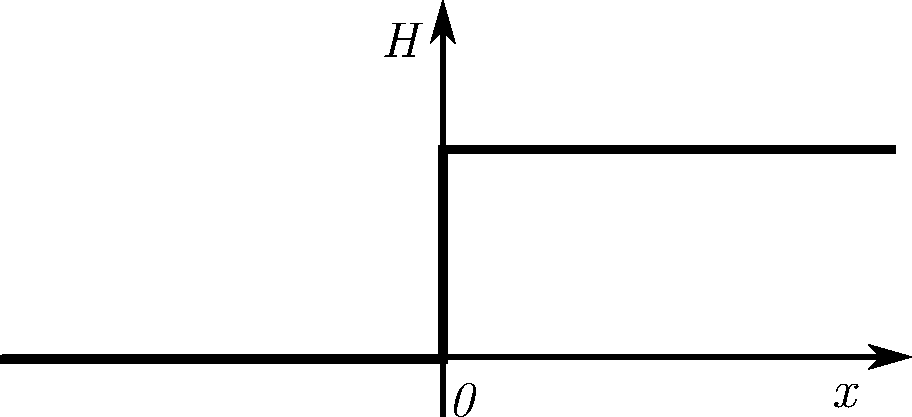
\includegraphics[width=0.6\textwidth]{heaviside.pdf}
	\caption{Funzione di Heaviside.}
	\label{heaviside2}
\end{figure}
\noindent
la soluzione fondamentale \`e
\[
	k(t,x)= \frac{1}{2c}(H(x+ct)- H(x-ct))
\]
Essa vale $1/(2c)$ nel dominio di influenza di vertice l'origine e $0$ altrove
\begin{figure}[H]
	\centering
	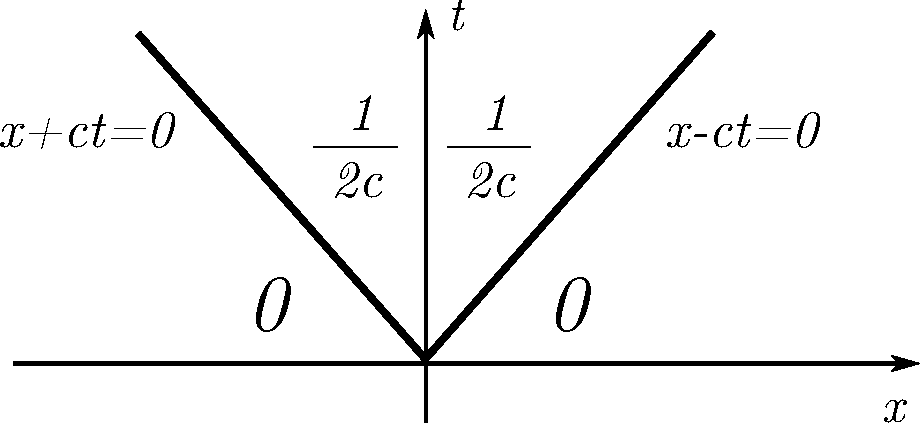
\includegraphics[width=0.6\textwidth]{fond_dom.pdf}
	\caption{Dominio di influenza per la soluzione fondamentale.}
	\label{fond_dom}
\end{figure}
\noindent
La singolarit\`a iniziale in  $x=0$ diventa una singolarit\`a di salto lungo la
caratteristica per l'origine.
Ad un tempo $t$ fissato, il grafico di $k(t,x)$
\begin{figure}[H]
	\centering
	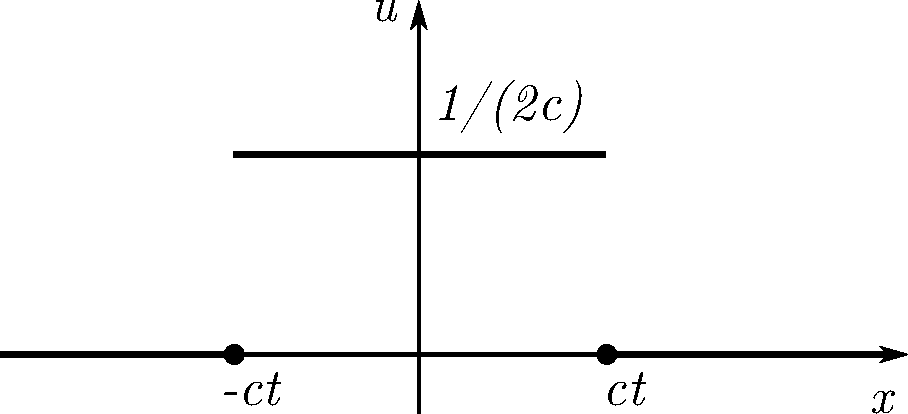
\includegraphics[width=0.6\textwidth]{fond_sol.pdf}
	\caption{Soluzione fondamentale.}
	\label{fond_sol}
\end{figure}
\noindent
Si noti che, fissare $u_t(0,x)=\delta(x)$ e $u(0,x)=0$,
significa anche a dire $u(t,0)= $ al gradino unitario in $x=0$, cio\`e
$u(t,0)=0$ con $t\leq 0$ e $u(t,0)=1/(2c)$ con $t>0$.\\
Abbiamo ottenuto la soluzione fondamentale dalla formula di D'Alambert.
Viceversa dalla espressione della soluzione fondamentale si pu\`o riottenere
tale formula.
Infatti, per traslazione, il problema
\[
	\left\{
	\begin{array}{l}
		u_{tt}-c^2u_{xx}=0\\
		u(0,x)=0\\
		u_t(0,x)=\delta_y
	\end{array}
	\right.
\]
\`e risolto da
\[
	k(t,x-y)= \frac{1}{2c}(H(x-y+ct)- H(x-y-ct)),
\]
funzione che vale $1/(2c)$ per $y-ct\leq x \leq y+ct$e che vale $0$ altrove.
La soluzione del problema generale
\[
	\left\{
	\begin{array}{l}
		u_{tt}-c^2u_{xx}=0\\
		u(0,x)=0\\
		u_t(0,x)=h(x)
	\end{array}
	\right.
\]
si ottiene per sovrapposizione tramite la convoluzione
\[
	u(t,x)= \intR k(t,x-y)h(y)dy
\]
Dunque
\[
	u(t,x)= \frac{1}{2c} \intR H(x-y+ct) h(y) dy -
	\frac{1}{2c} \intR H(x-y-ct) h(y) dy
\]
\[
	=\frac{1}{2c} \int_{-\infty}^{x+ct} h(y) dy -
	\frac{1}{2c} \int_{-\infty}^{x-ct} h(y) dy
	=\frac{1}{2c} \int_{x-ct}^{x+ct} h(y) dy
\]
che \`e la formula di D'Alambert per $u(0,x)=g(x)=0$. Abbiamo gi\`a visto che
la formula fondamentale si deduce da questo caso $g=0$.

%
\addcontentsline{toc}{chapter}{Elenco delle figure}
\listoffigures
%
\end{document}
